% ==============================================================================
\chapter{Thin sensors studies}
\label{ch:ThinSensorsStudies}
%==============================================================================    

%% --------------------------------------------- %%
\section{Samples and sensors geometries}
Operating conditions for the Timepix3 readout ASICs:
\begin{itemize}
\item I\textsubscript{krum} DAC is set to 10.
\item TOT clock frequency: $40\,\megahertz$
\item VFBK: 150
\end{itemize}


 For most of the measurements, the DUT is perpendicular to the beam. A
 scan was done on the bias voltage and the threshold of the DUT. The
 bias scan allows to obtain the depletion voltage.

%% --------------------------------------------- %%
\section{Test-beam results for thin sensors}

\subsection{Bias scan}

The total TOT of all cluster sizes is fitted with a landau function
convoluted with a Gaussian. The fit is done using RooFit and an
example is given in \cref{fig:W2_J5_1998_totalTOT_langauFit}. The MPV
of the Landau and the error on the fit are plotted versus the square
root of the bias voltage.

\begin{figure}[htbp] 
  \centering
  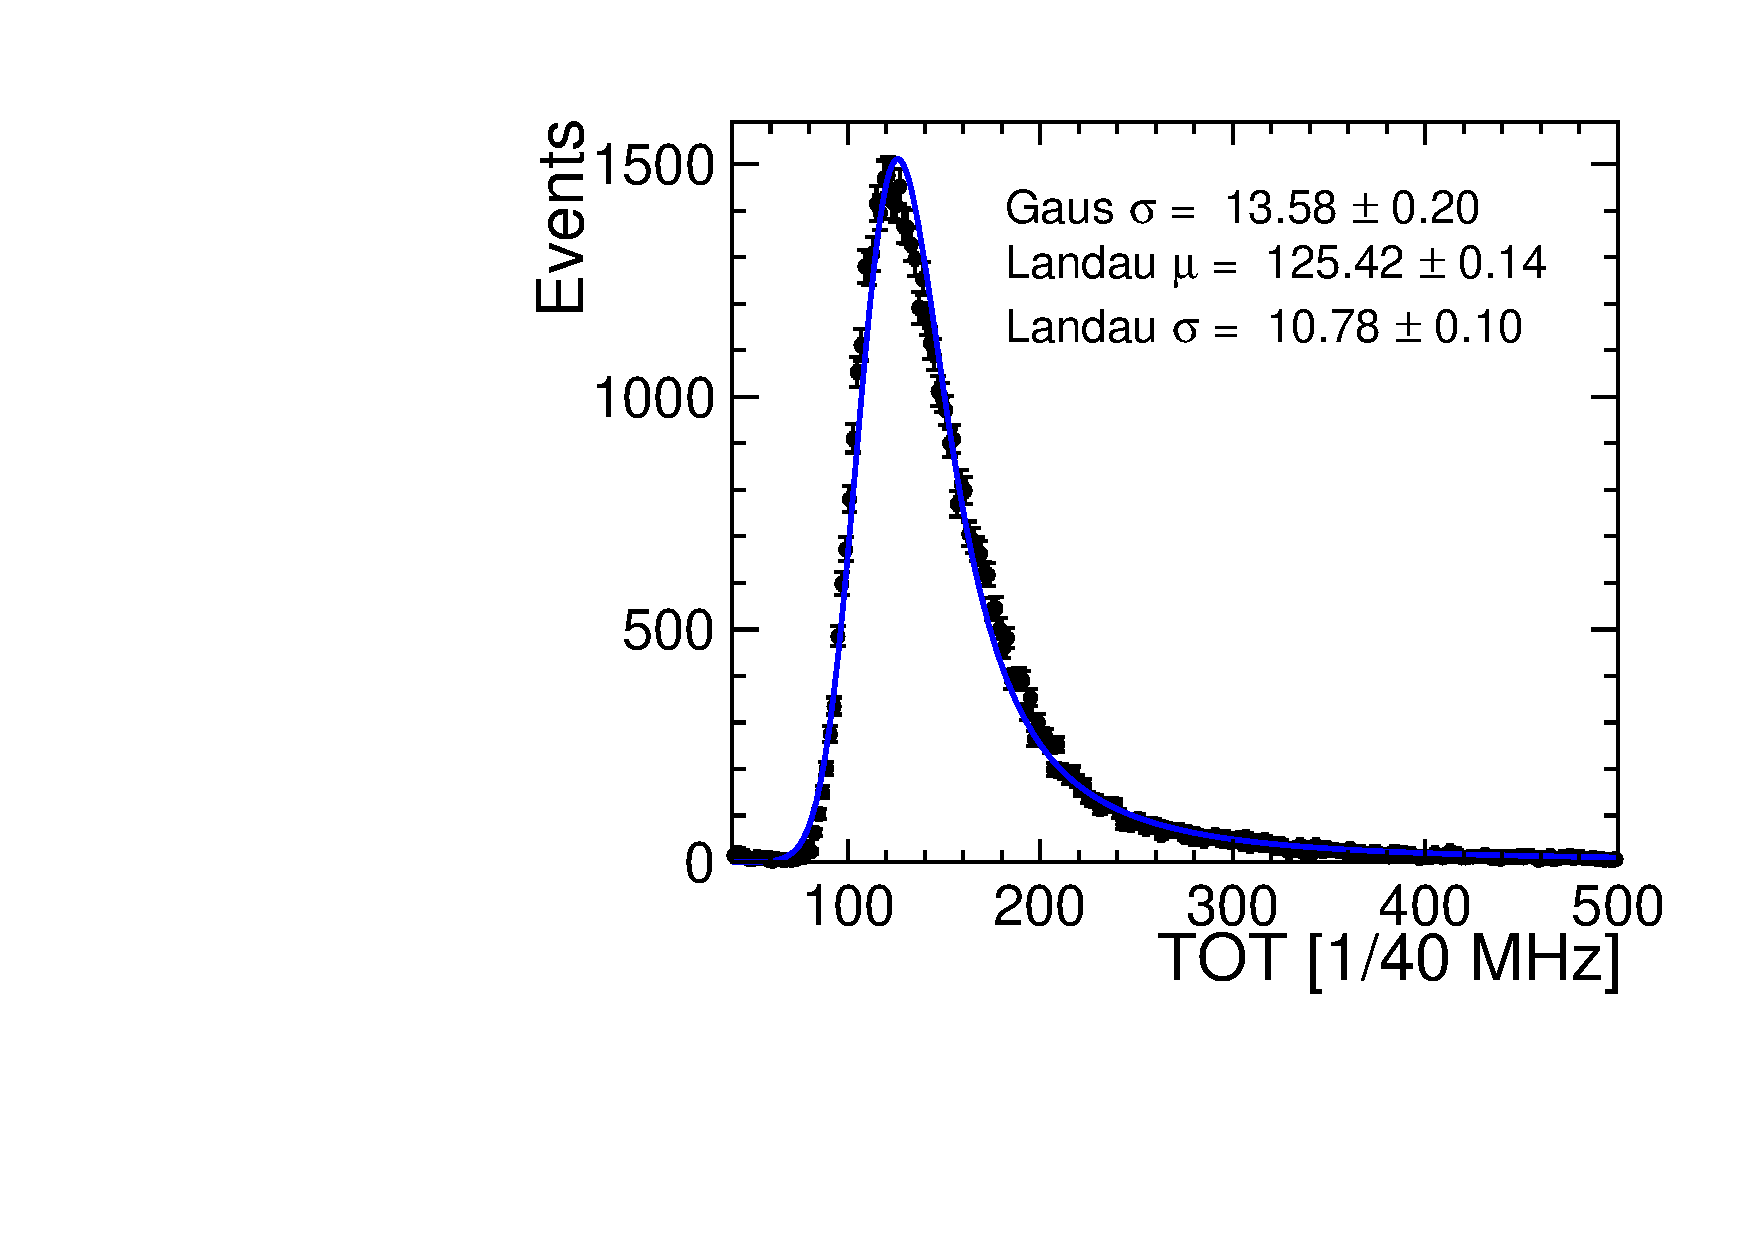
\includegraphics[width=0.5\textwidth]{./figures/TestBeam/W2_J5_totalTOT_Langau_run1998.pdf}
  \caption{W2\_J5: Vbias=95 V}
  \label{fig:W2_J5_1998_totalTOT_langauFit}
\end{figure}

\begin{table}[htbp]
  \centering
  \caption{Measured depletion voltage}
  \label{tab:depletionVoltage}
  \begin{tabular}{lcccc}
    \toprule
    Assembly & Thickness [\micron] & Sensor type & Nominal voltage [V] & Depletion voltage [V] \\
    \midrule
    20-NGR  & 50 & n-in-p & -15 & $<$-9.47 \\
    23-FGR & 50 & n-in-p & -15 & $<$-6.32 \\
    28-GNDGR & 50 & n-in-p & -15 & $<$-7.19\\
    55-GNDGR & 50 & n-in-p & -15 & $<$-5.43\\ \hline
    55-GNDGR-100 & 100 & n-in-p & -20 & -10.82 \\ \hline
    55-GNDGR-150 & 150 & n-in-p & -30 & -14.86 \\ \hline
    W2\_J5       & 300 & p-in-n & 100 & 63.23 \\ 
    \bottomrule
  \end{tabular}
\end{table}


\subsection{Threshold scan}

\subsection{Resolution vs. thickness}
\begin{figure}[htbp] \centering
  \begin{subfigure}[b]{0.45\textwidth}
    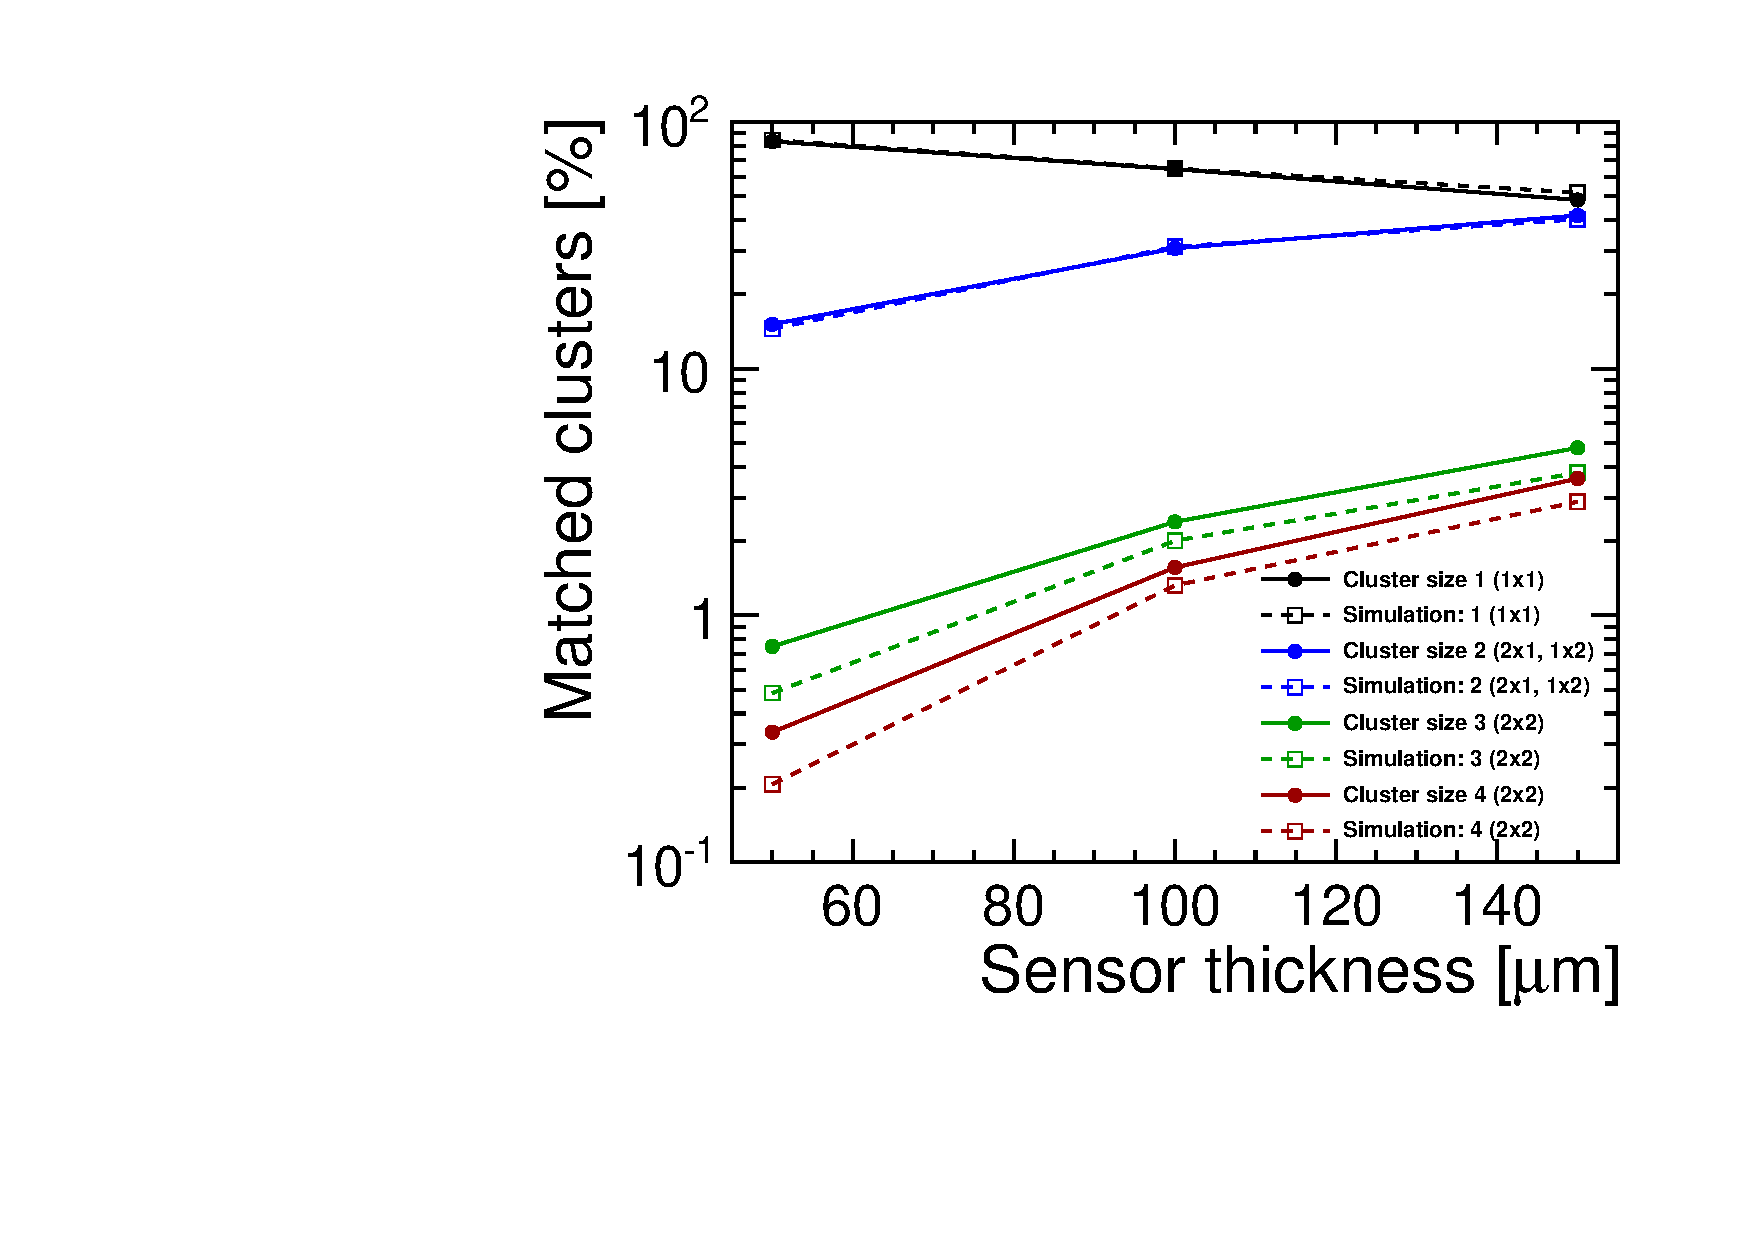
\includegraphics[width=\textwidth]{./figures/TestBeam/cluSize_vs_thickness.pdf}
    \caption{}
  \end{subfigure} \hfill
  \begin{subfigure}[b]{0.45\textwidth}
    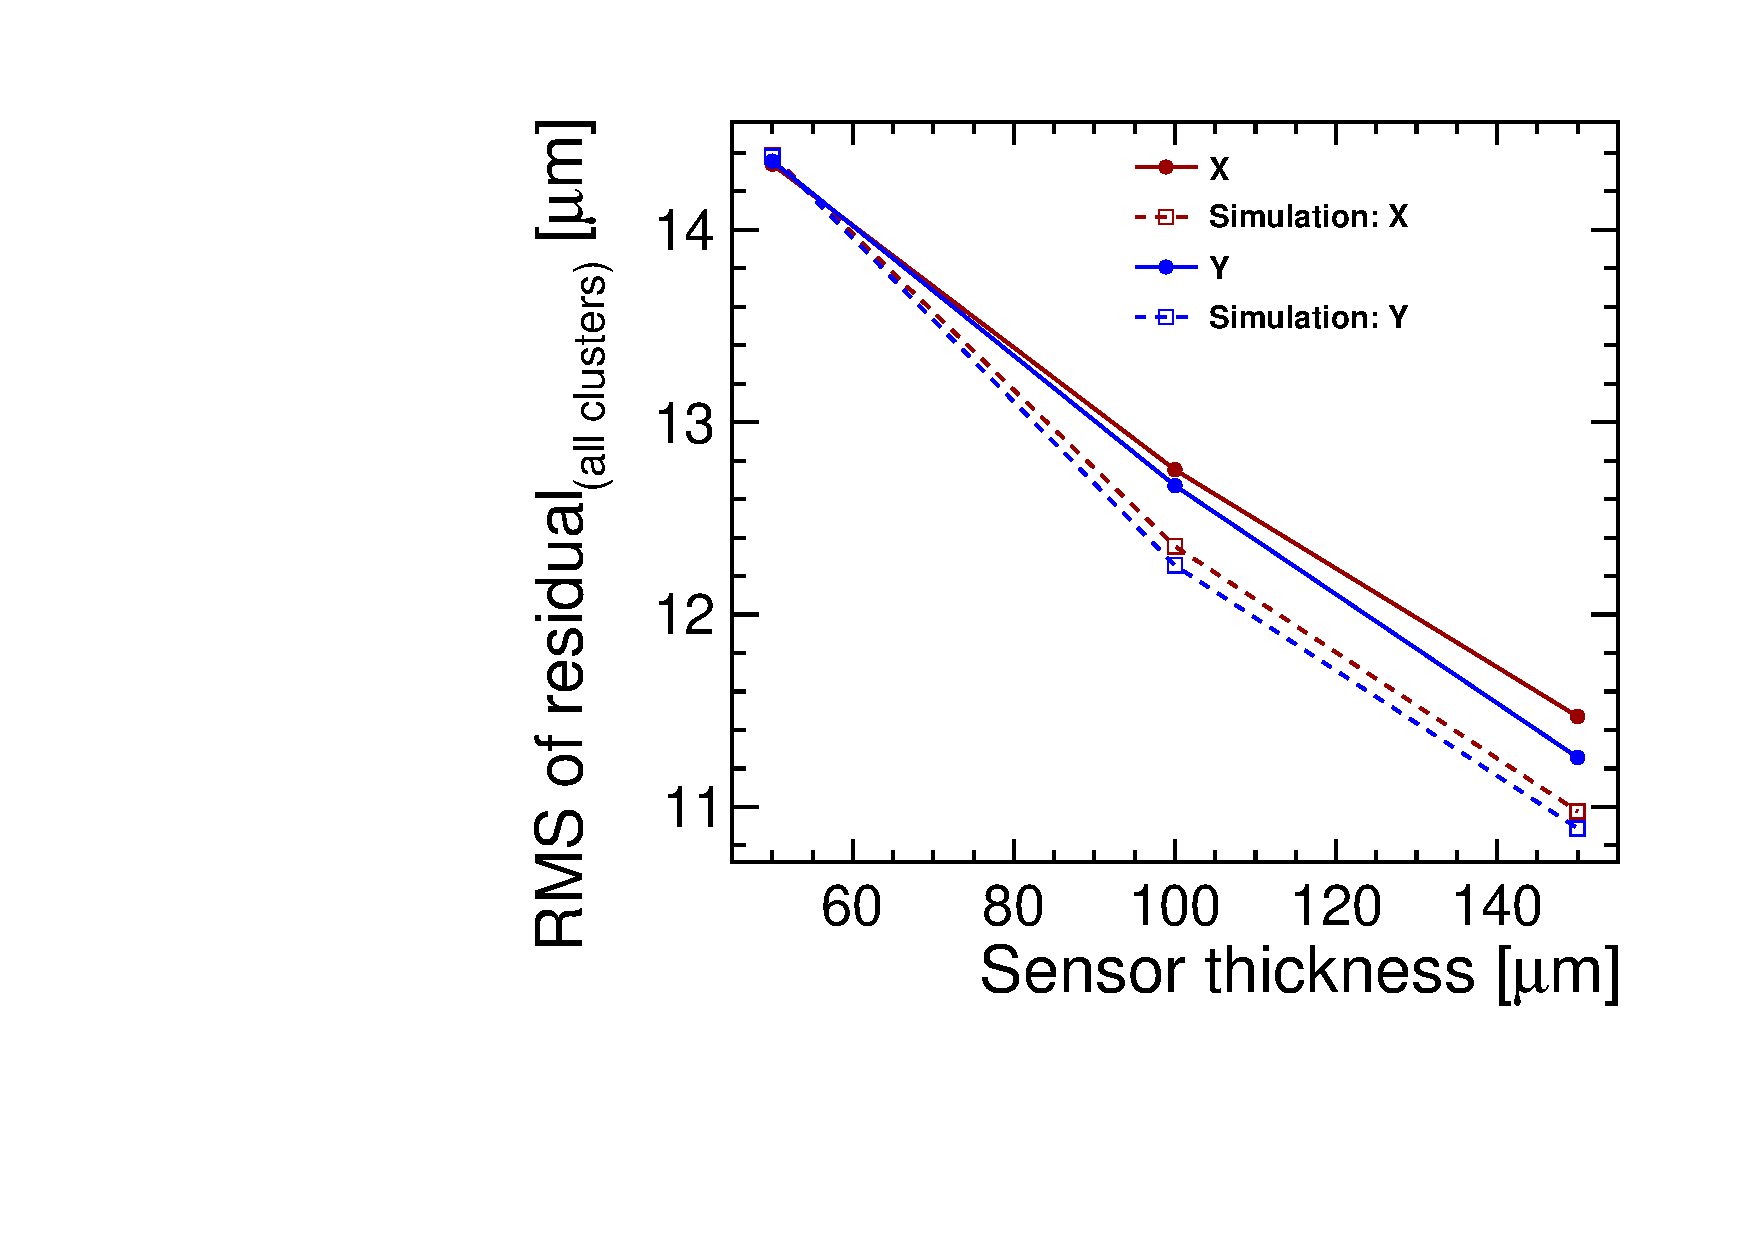
\includegraphics[width=\textwidth]{./figures/TestBeam/residuals_vs_thickness.pdf}
    \caption{}
  \end{subfigure}
  \caption{Cluster size and residuals vs. thickness (run 2003 for 300 um thick sensor was taken at 70 V).}
  \label{fig:clusize_residuals_vs_thickness}
\end{figure}


\subsection{Efficiency vs. thickness}

The efficiency as a function of the threshold is shown in \cref{fig:efficiency_VS_Threshold}.

\begin{figure}[htbp] 
  \centering
  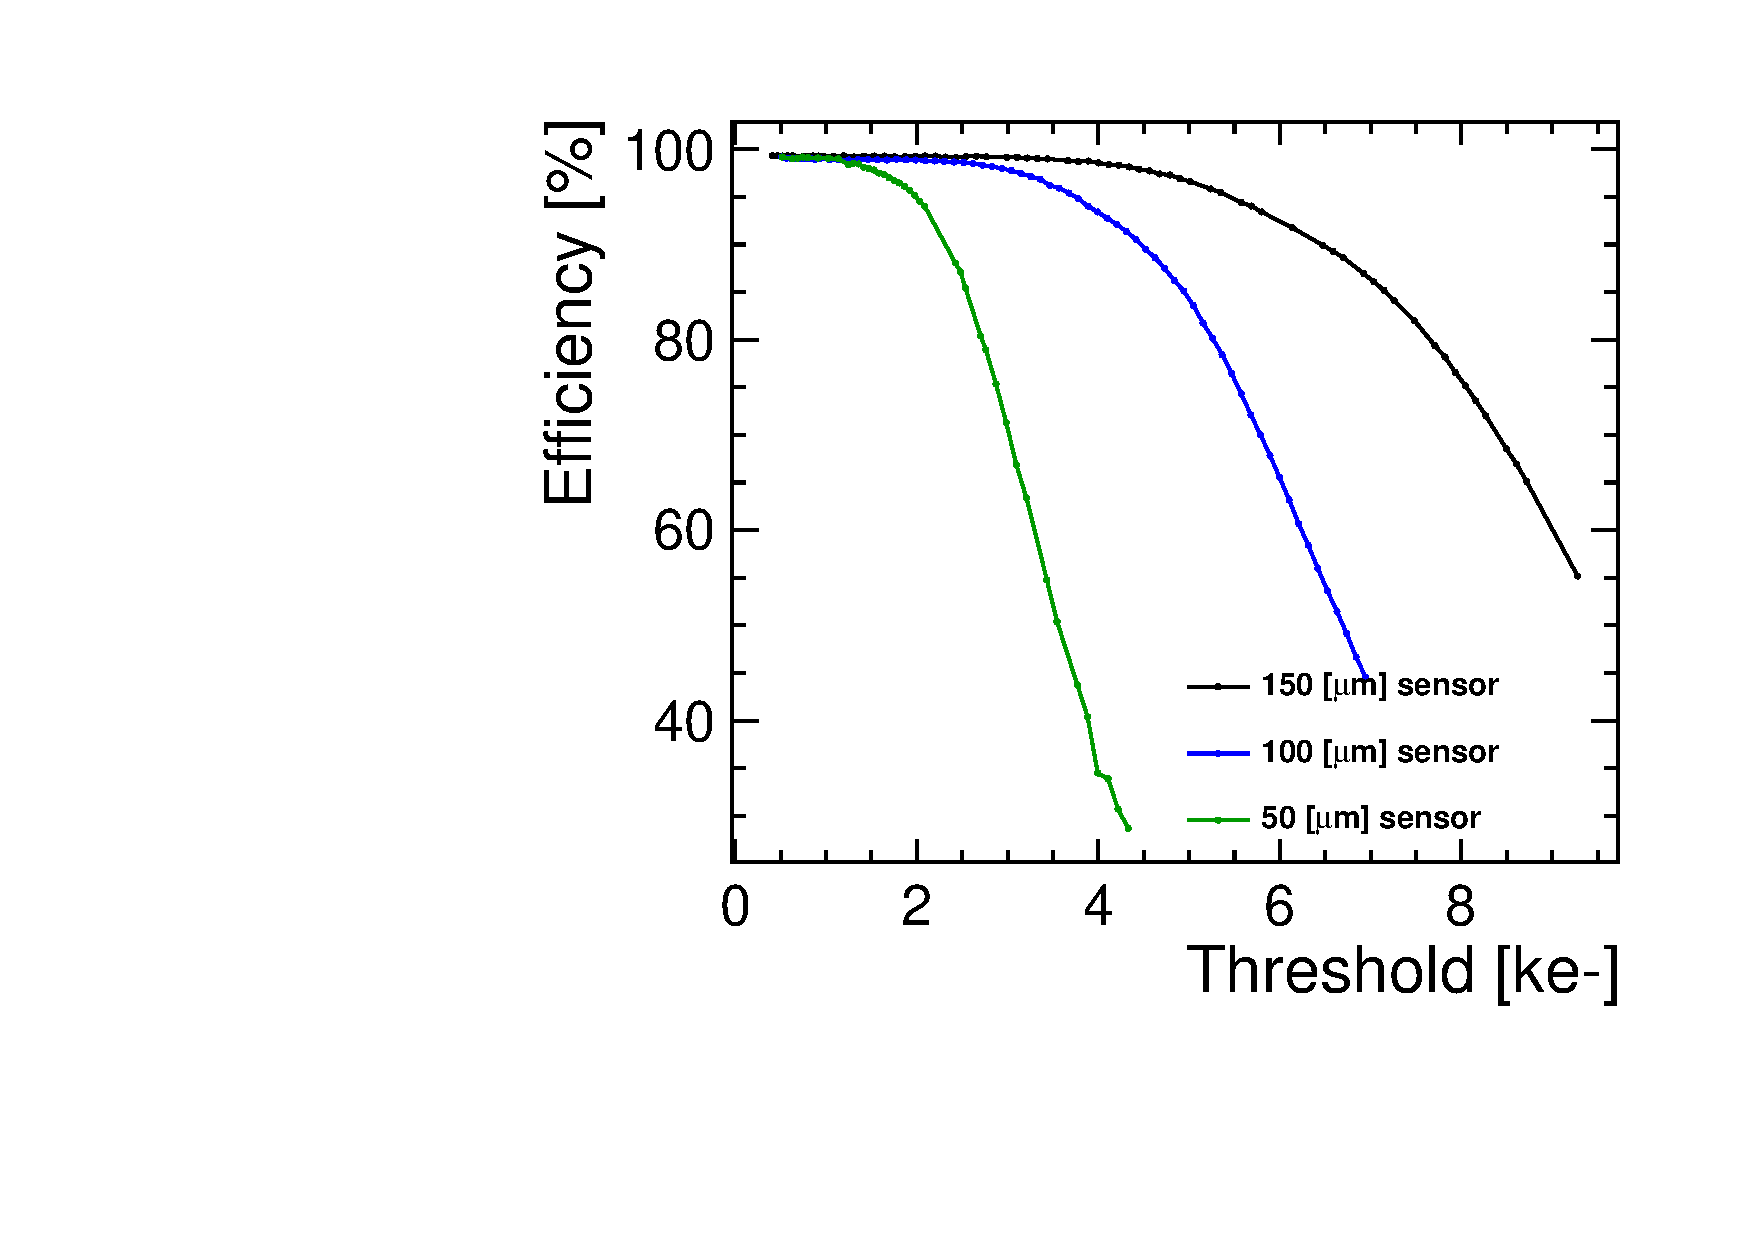
\includegraphics[width=0.5\textwidth]{./figures/TestBeam/Efficiency_vs_THL.pdf}
  \caption{Efficiency vs. threshold: W2\_J5 is missing.}
  \label{fig:efficiency_VS_Threshold}
\end{figure}


%% --------------------------------------------- %%
\section{Validation of the simulation}
%% --------------------------------------------- %%
\section{Extrapolation to smaller pixels (CLICpix)}

%% %% --------------------------------------------- %%
%% \begin{figure}[htbp] \centering
%%   \begin{subfigure}[b]{0.45\textwidth}
%%     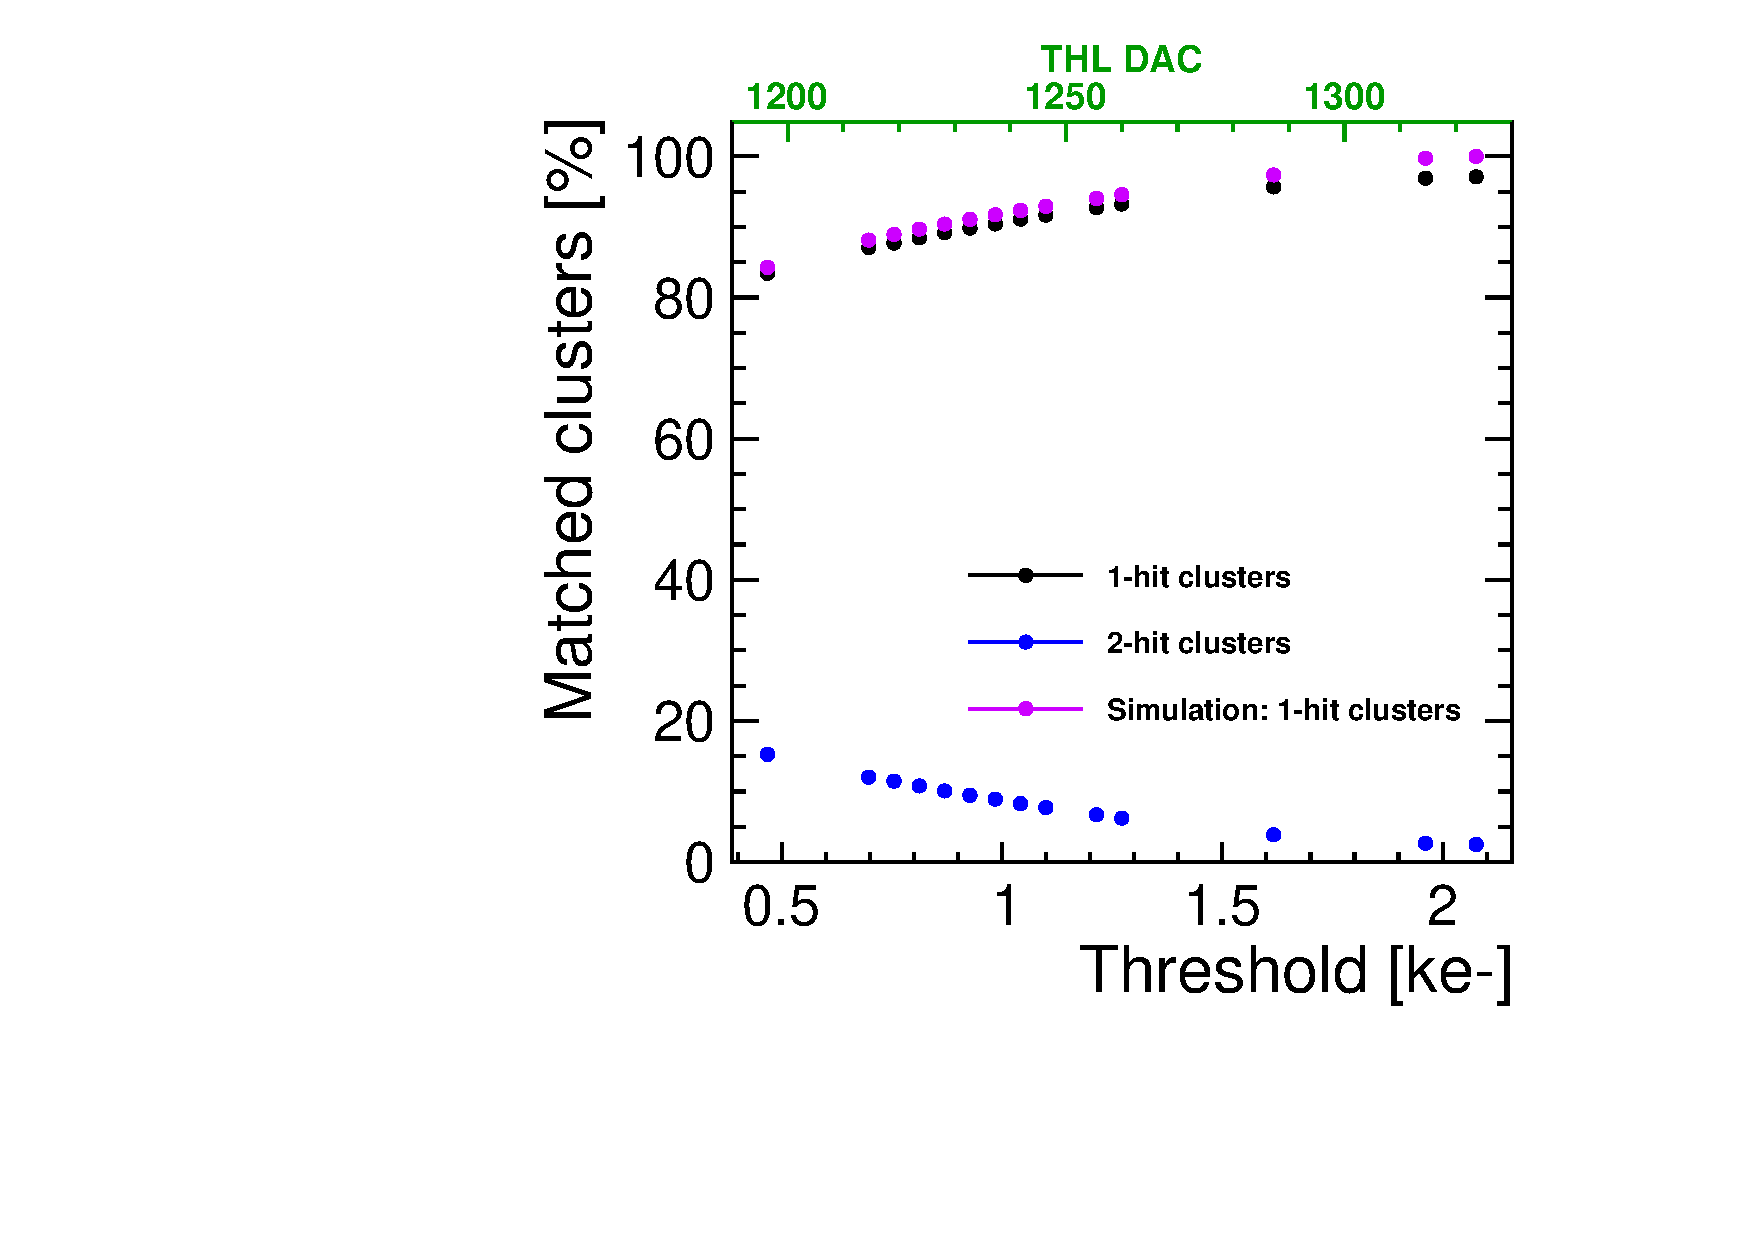
\includegraphics[width=\textwidth]{./figures/TestBeam/ThresholdScan_W0019_G07.pdf}
%%     \caption{}
%%   \end{subfigure} \hfill
%%   \begin{subfigure}[b]{0.45\textwidth}
%%     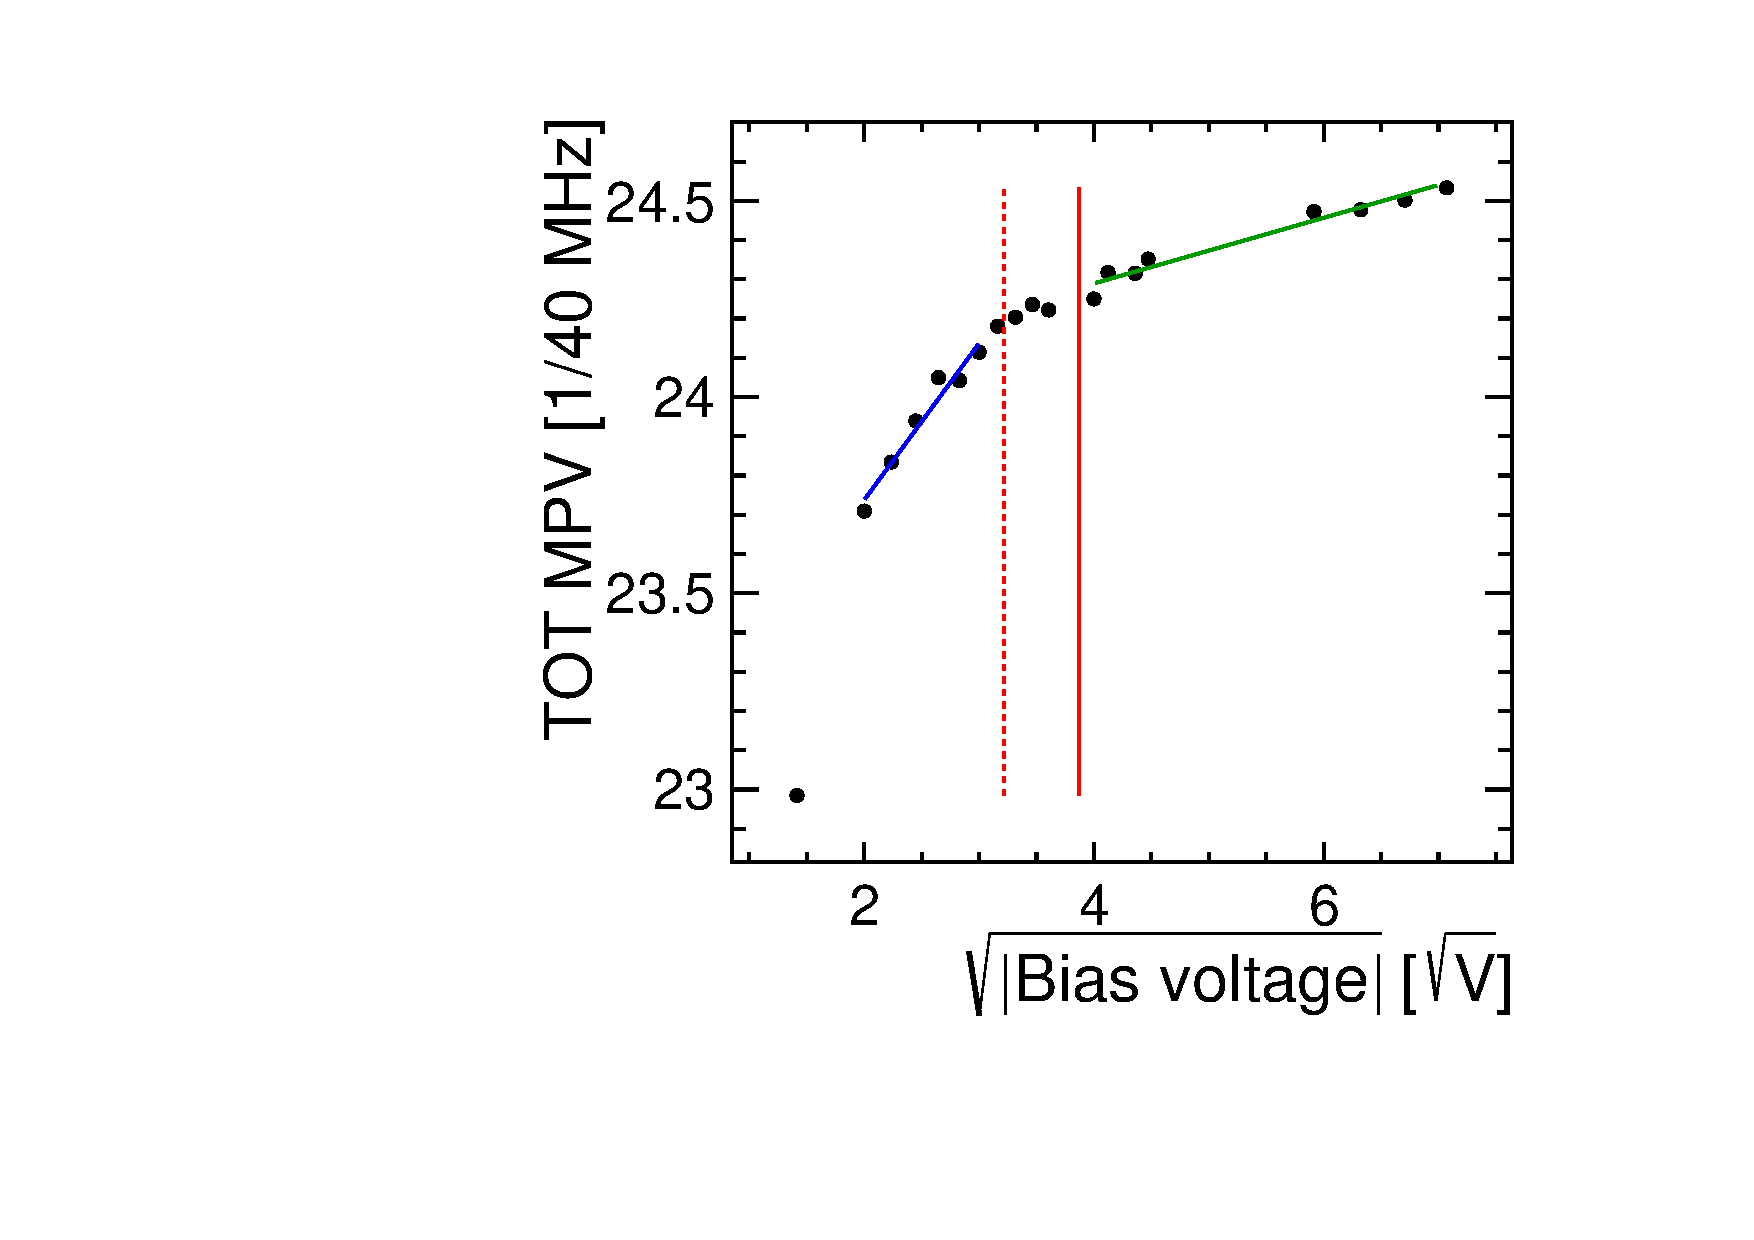
\includegraphics[width=\textwidth]{./figures/TestBeam/depletionVoltage_W0019_G07.pdf}
%%     \caption{}
%%   \end{subfigure}
%%   \caption{20-NGR (W19\_G7): bias and voltage scan.}
%%   \label{fig:Timepix3_THLscan_Vdep_G7}
%% \end{figure}

%% \begin{figure}[htbp] \centering
%%   \begin{subfigure}[b]{0.45\textwidth}
%%     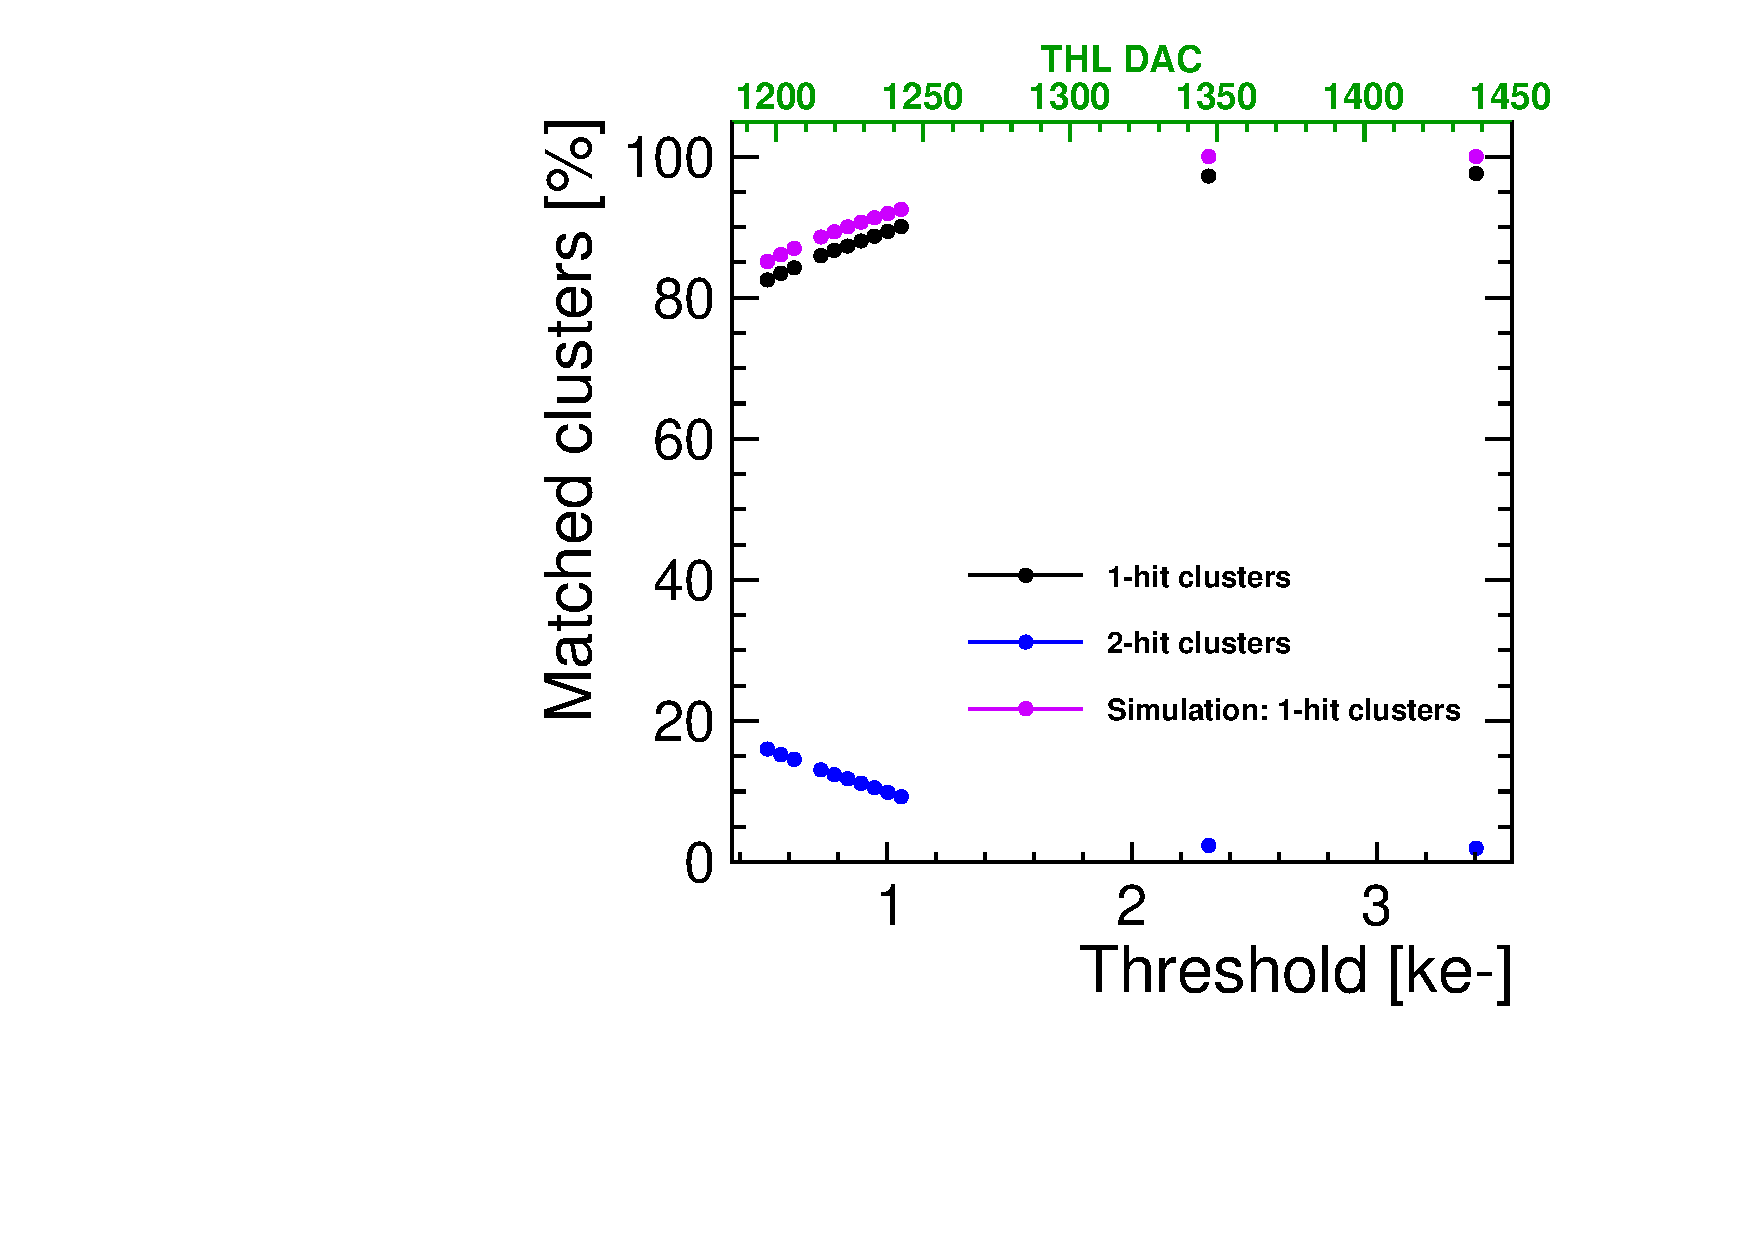
\includegraphics[width=\textwidth]{./figures/TestBeam/ThresholdScan_W0019_F07.pdf}
%%     \caption{}
%%   \end{subfigure} \hfill
%%   \begin{subfigure}[b]{0.45\textwidth}
%%     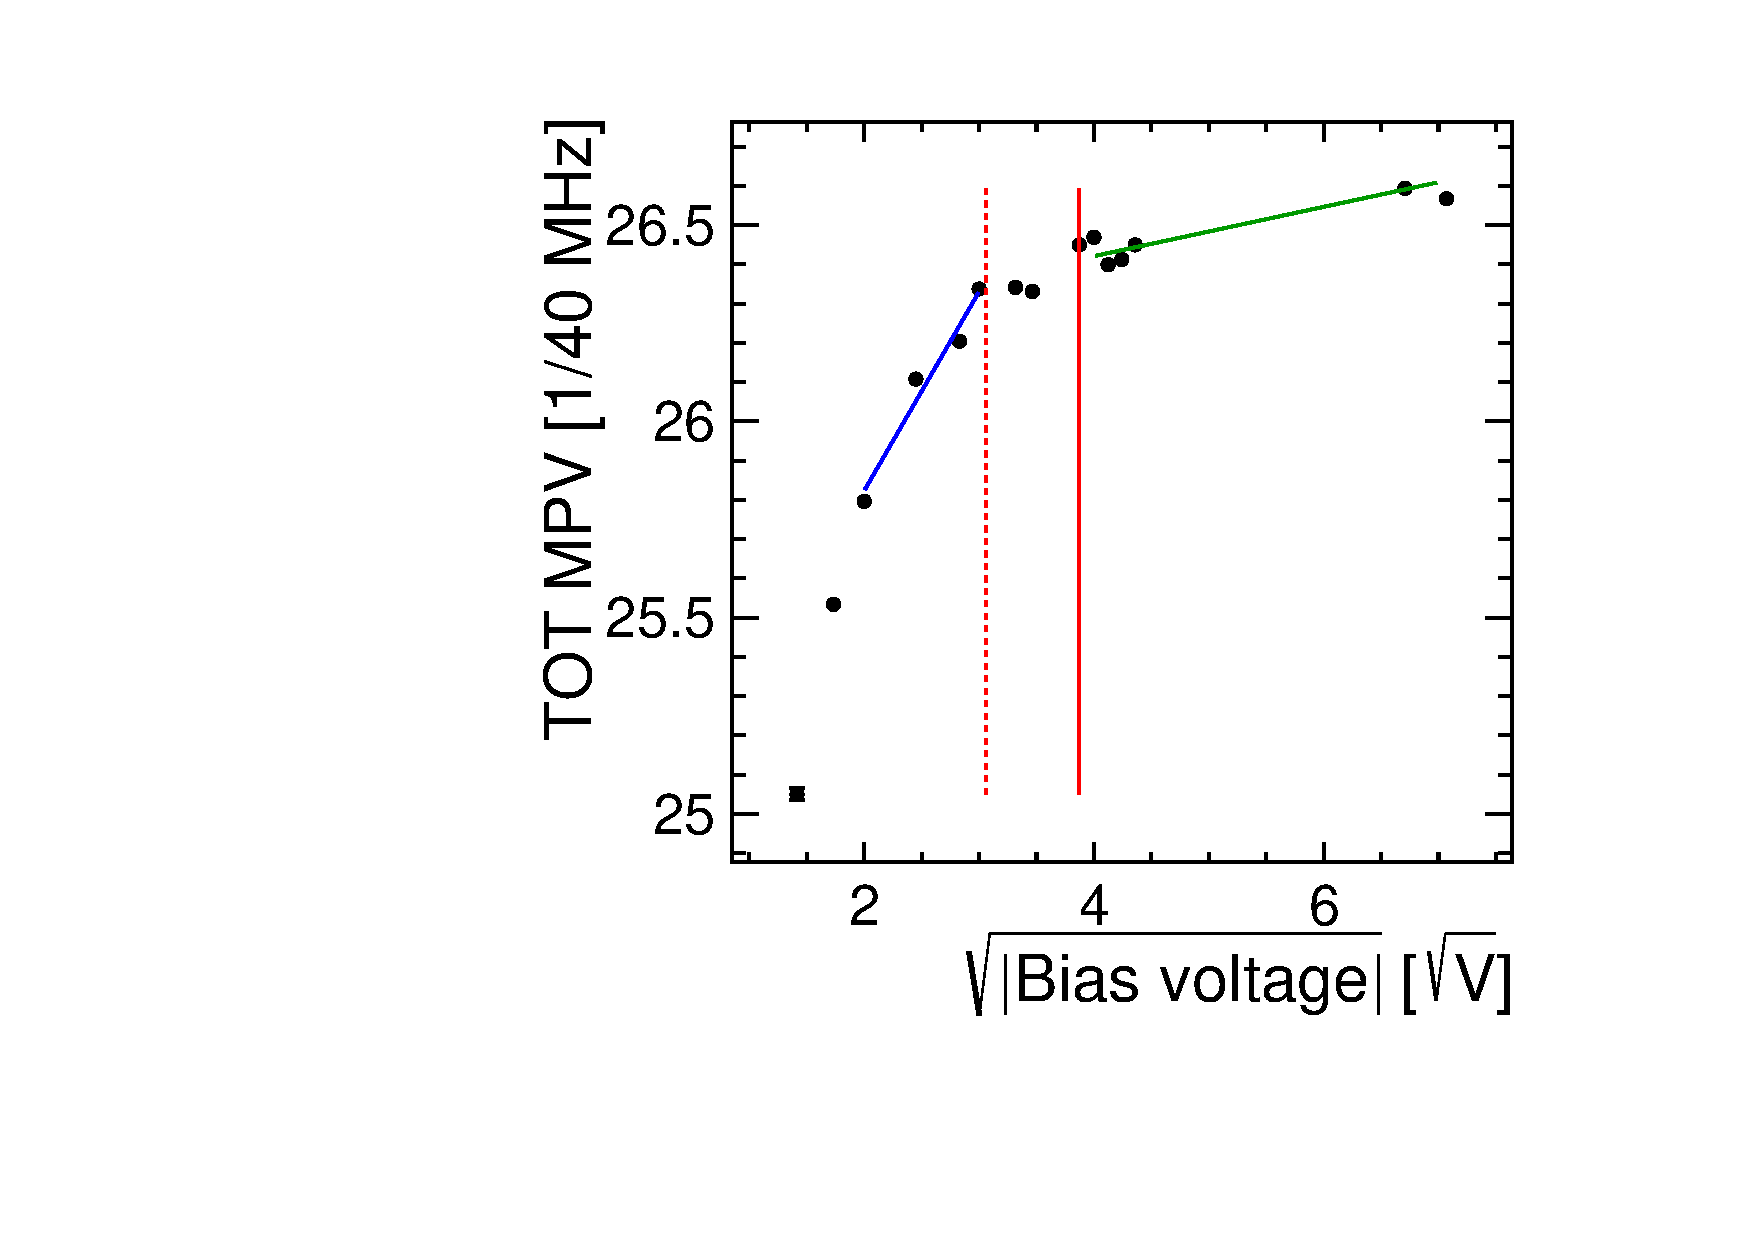
\includegraphics[width=\textwidth]{./figures/TestBeam/depletionVoltage_W0019_F07.pdf}
%%     \caption{}
%%   \end{subfigure}
%%   \caption{23-FGR (W19\_F7): bias and voltage scan.}
%%   \label{fig:Timepix3_THLscan_Vdep_F7}
%% \end{figure}

%% \begin{figure}[htbp] \centering
%%   \begin{subfigure}[b]{0.45\textwidth}
%%     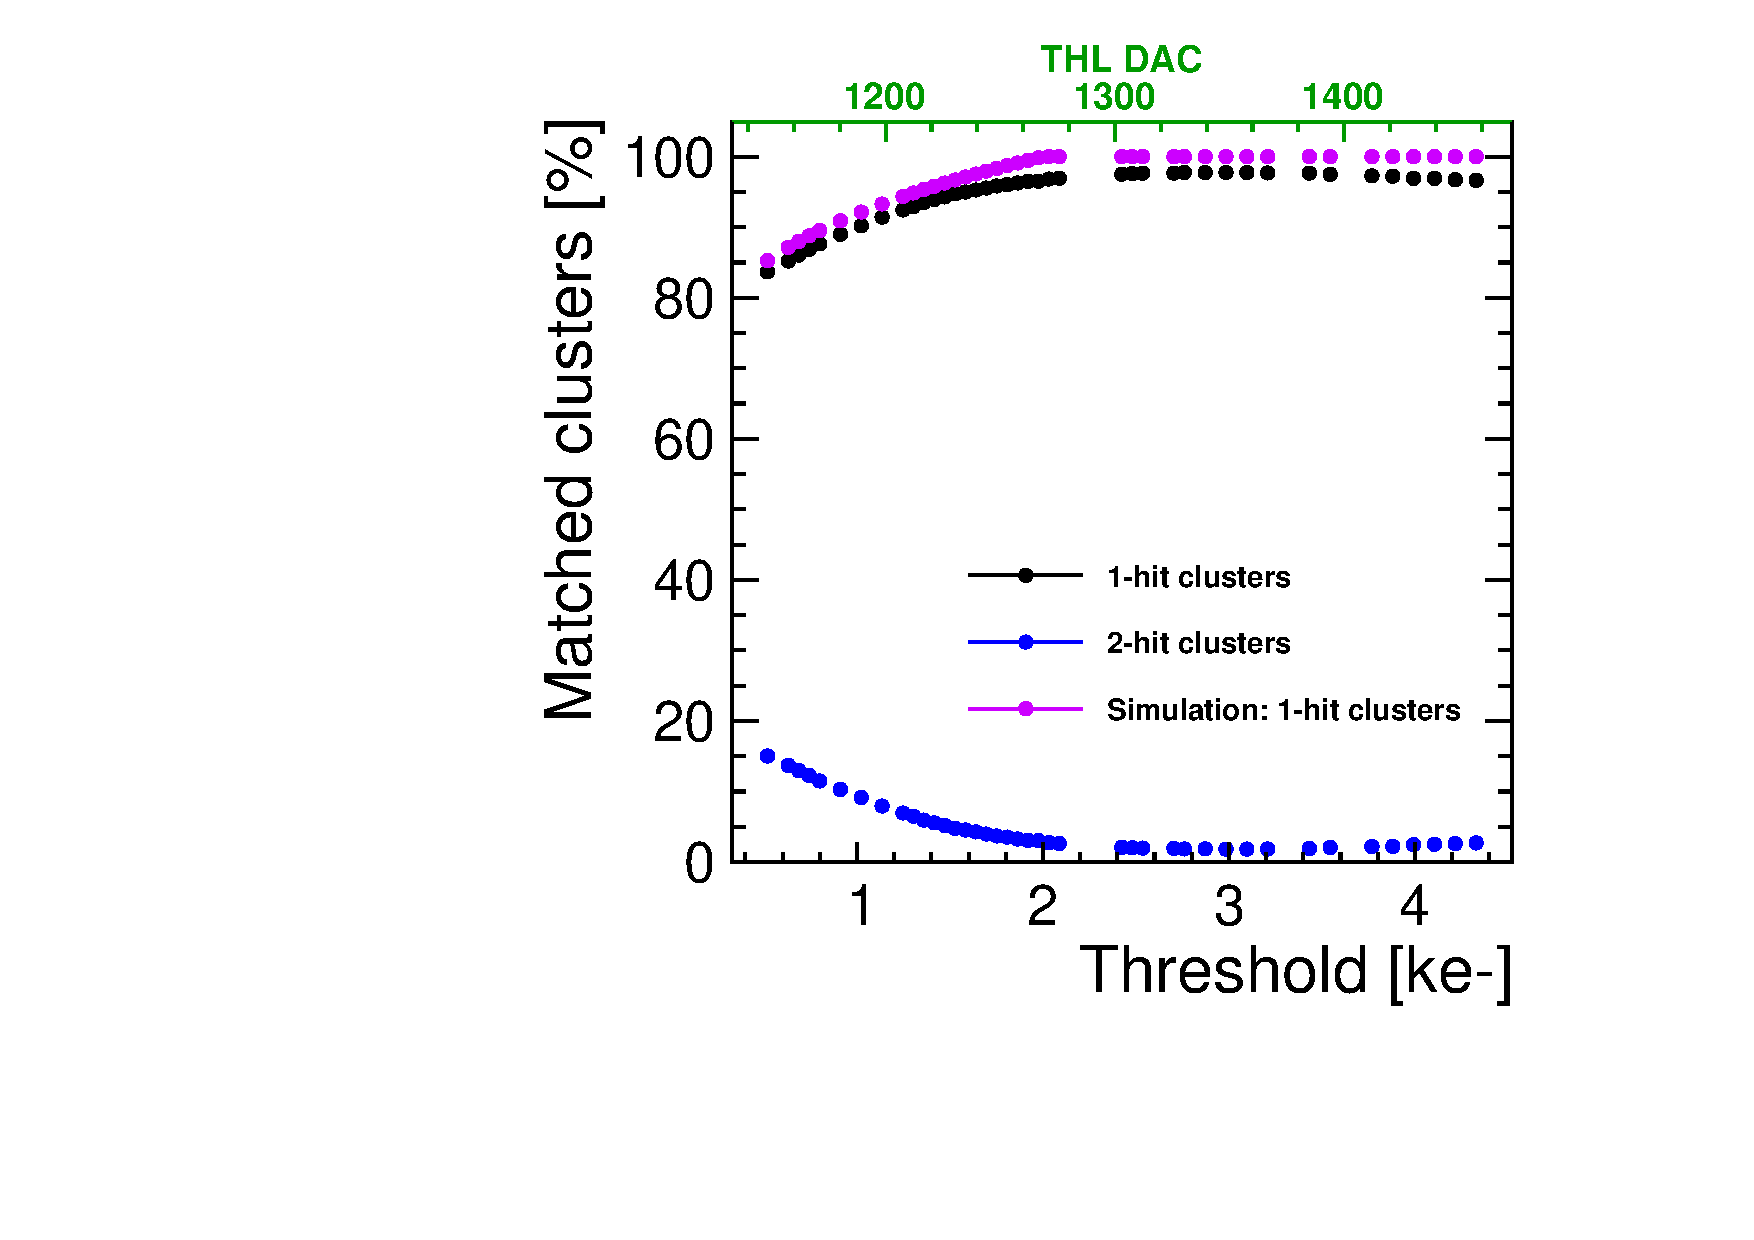
\includegraphics[width=\textwidth]{./figures/TestBeam/ThresholdScan_W0019_L08.pdf}
%%     \caption{}
%%   \end{subfigure} \hfill
%%   \begin{subfigure}[b]{0.45\textwidth}
%%     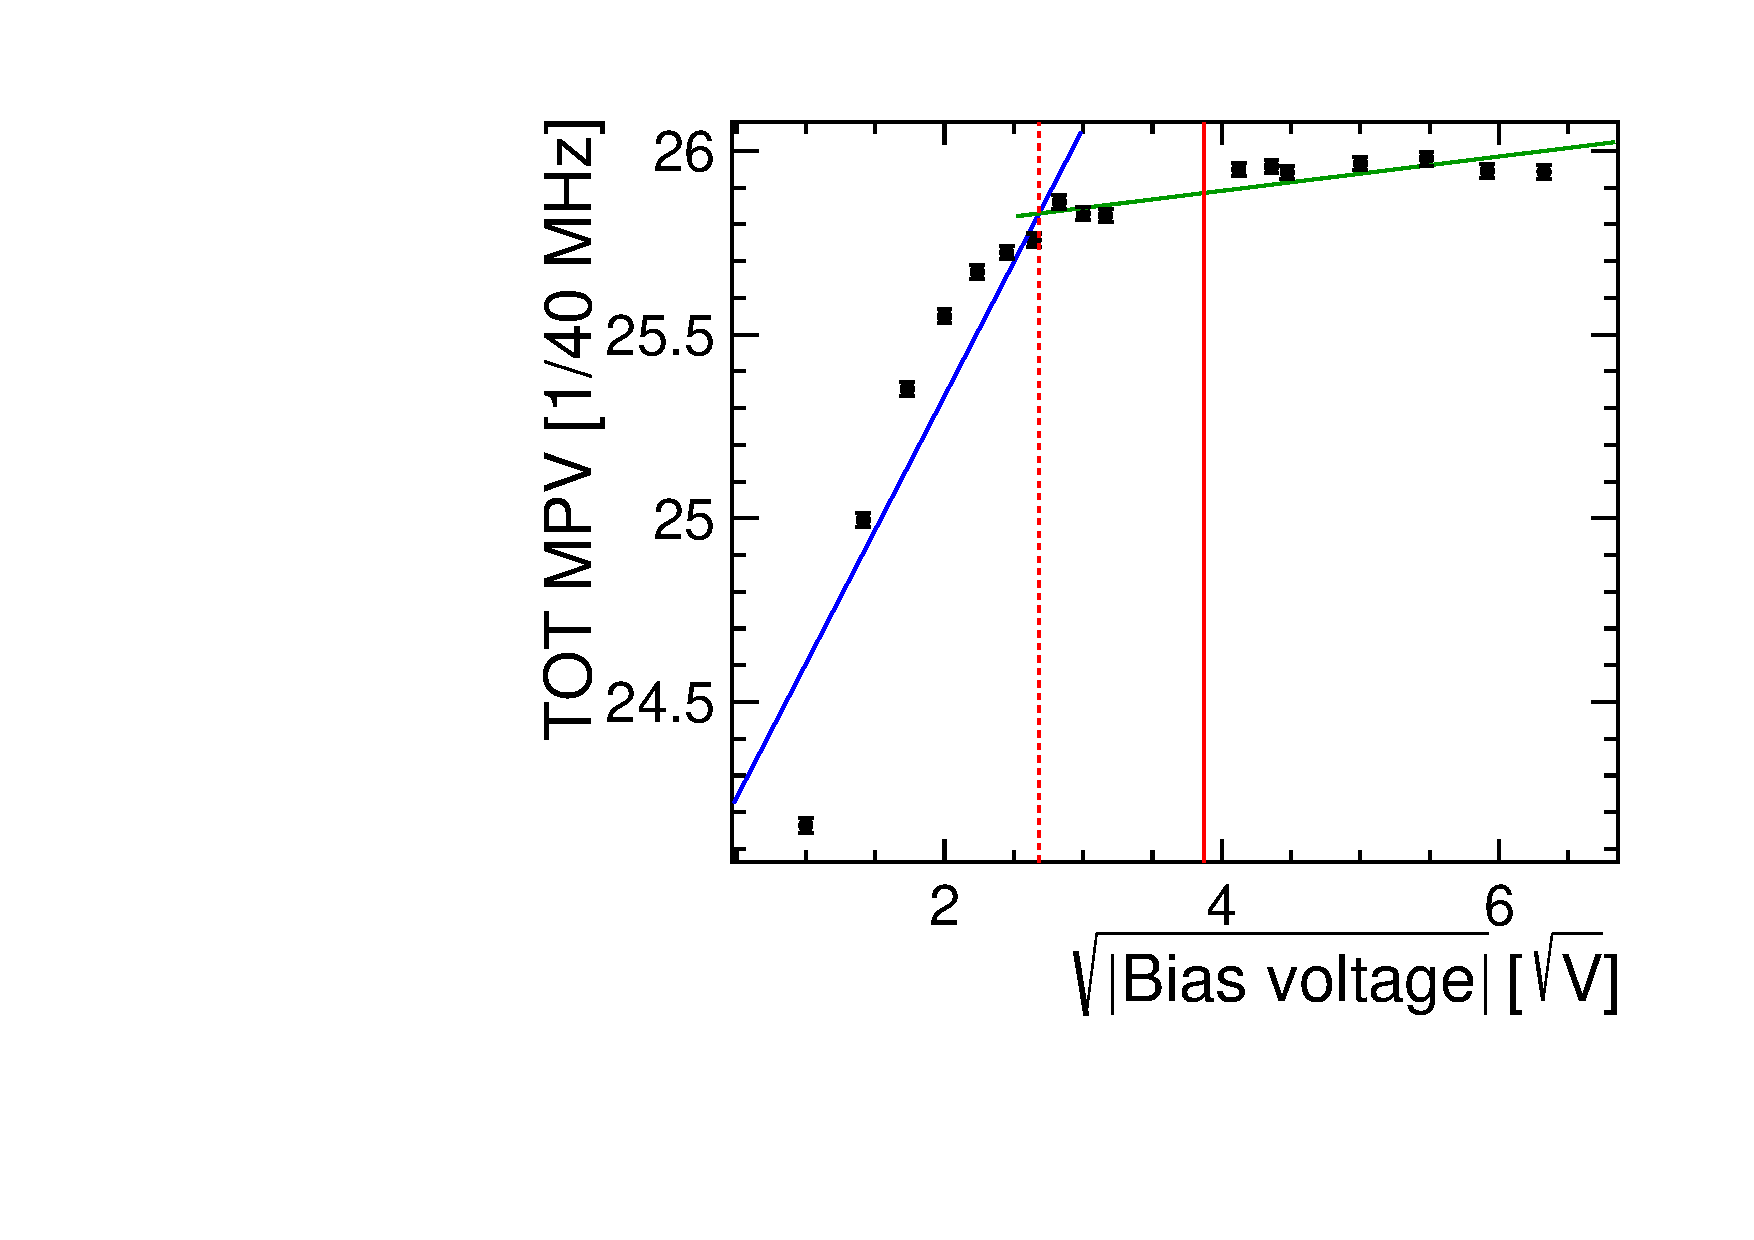
\includegraphics[width=\textwidth]{./figures/TestBeam/depletionVoltage_W0019_L08.pdf}
%%     \caption{}
%%   \end{subfigure}
%%   \caption{28-GNDGR (W19\_L8): bias and voltage scan.}
%%   \label{fig:Timepix3_THLscan_Vdep_L8}
%% \end{figure}


%% \begin{figure}[htbp] \centering
%%   \begin{subfigure}[b]{0.45\textwidth}
%%     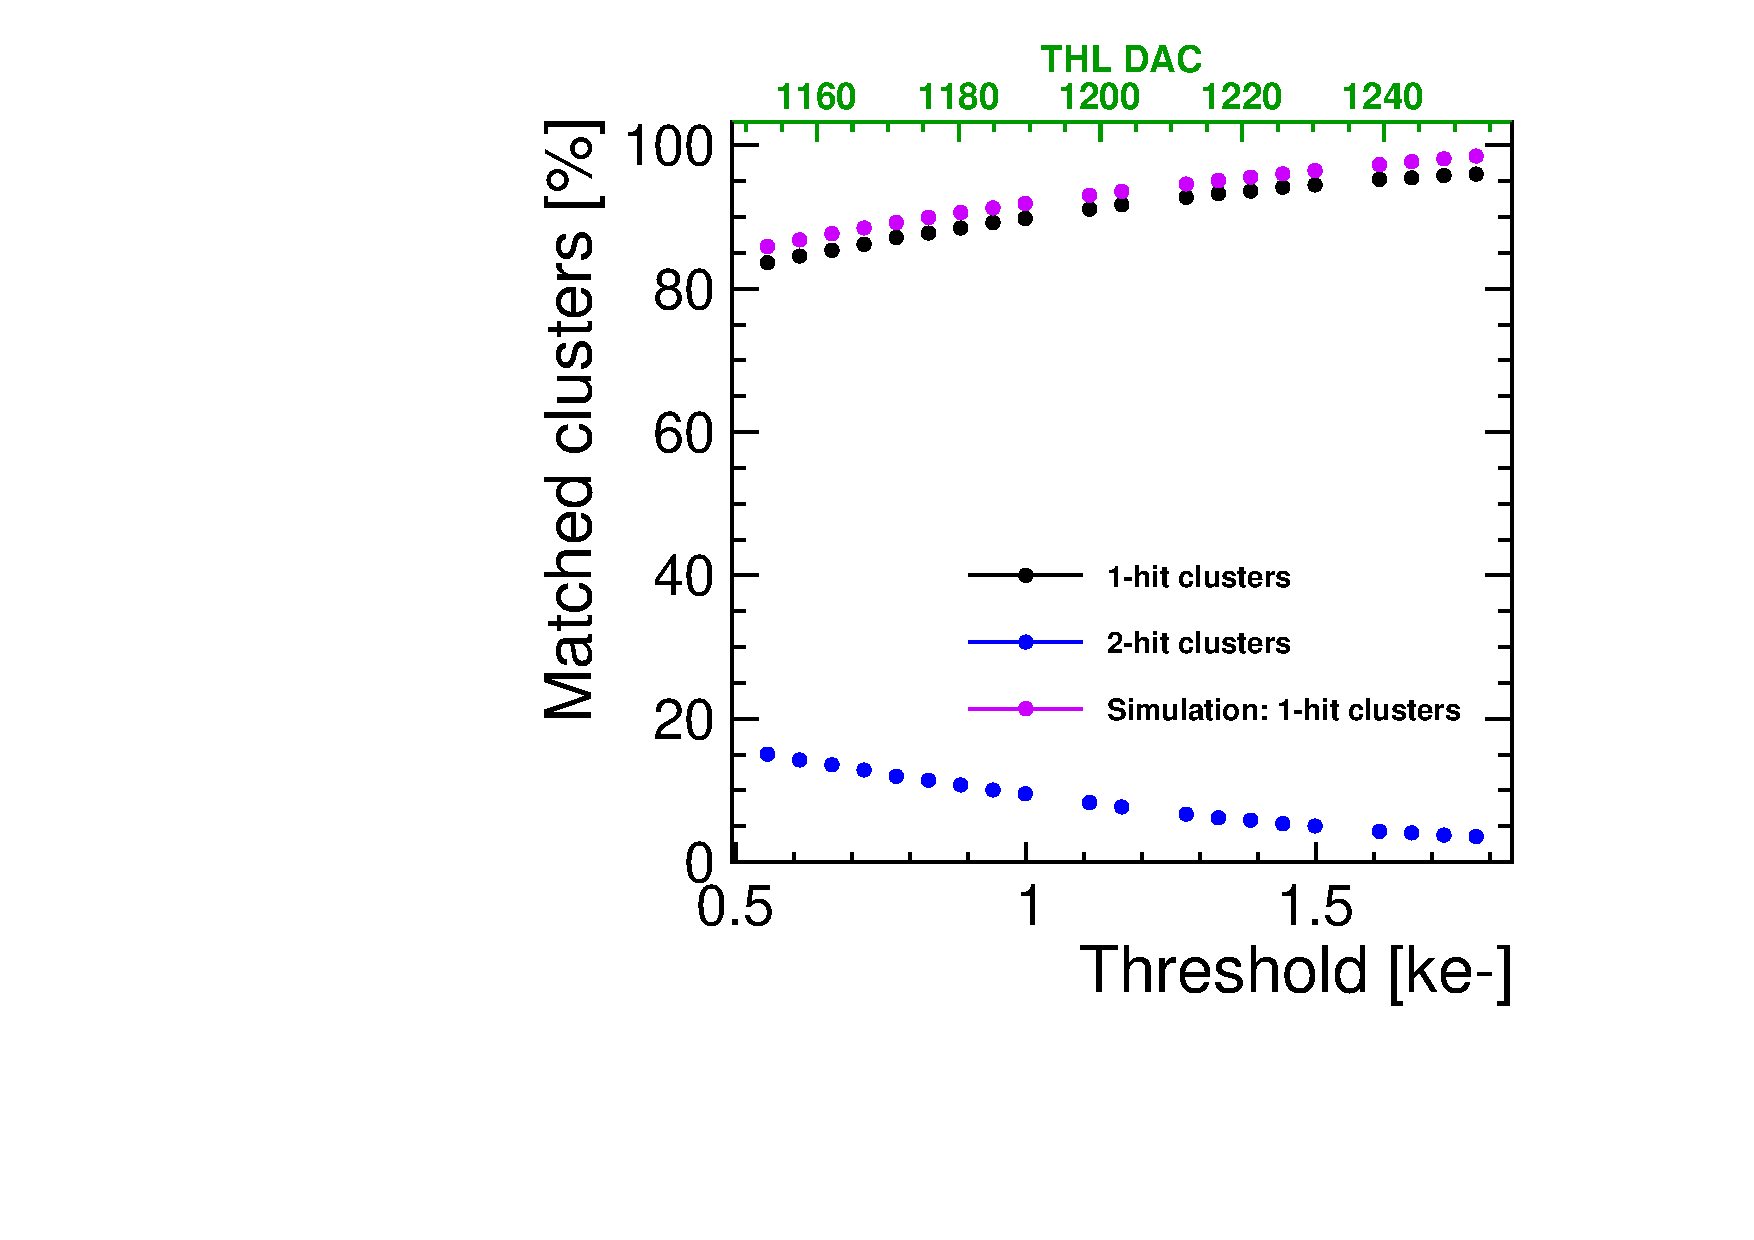
\includegraphics[width=\textwidth]{./figures/TestBeam/ThresholdScan_W0019_C07.pdf}
%%     \caption{}
%%   \end{subfigure} \hfill
%%   \begin{subfigure}[b]{0.45\textwidth}
%%     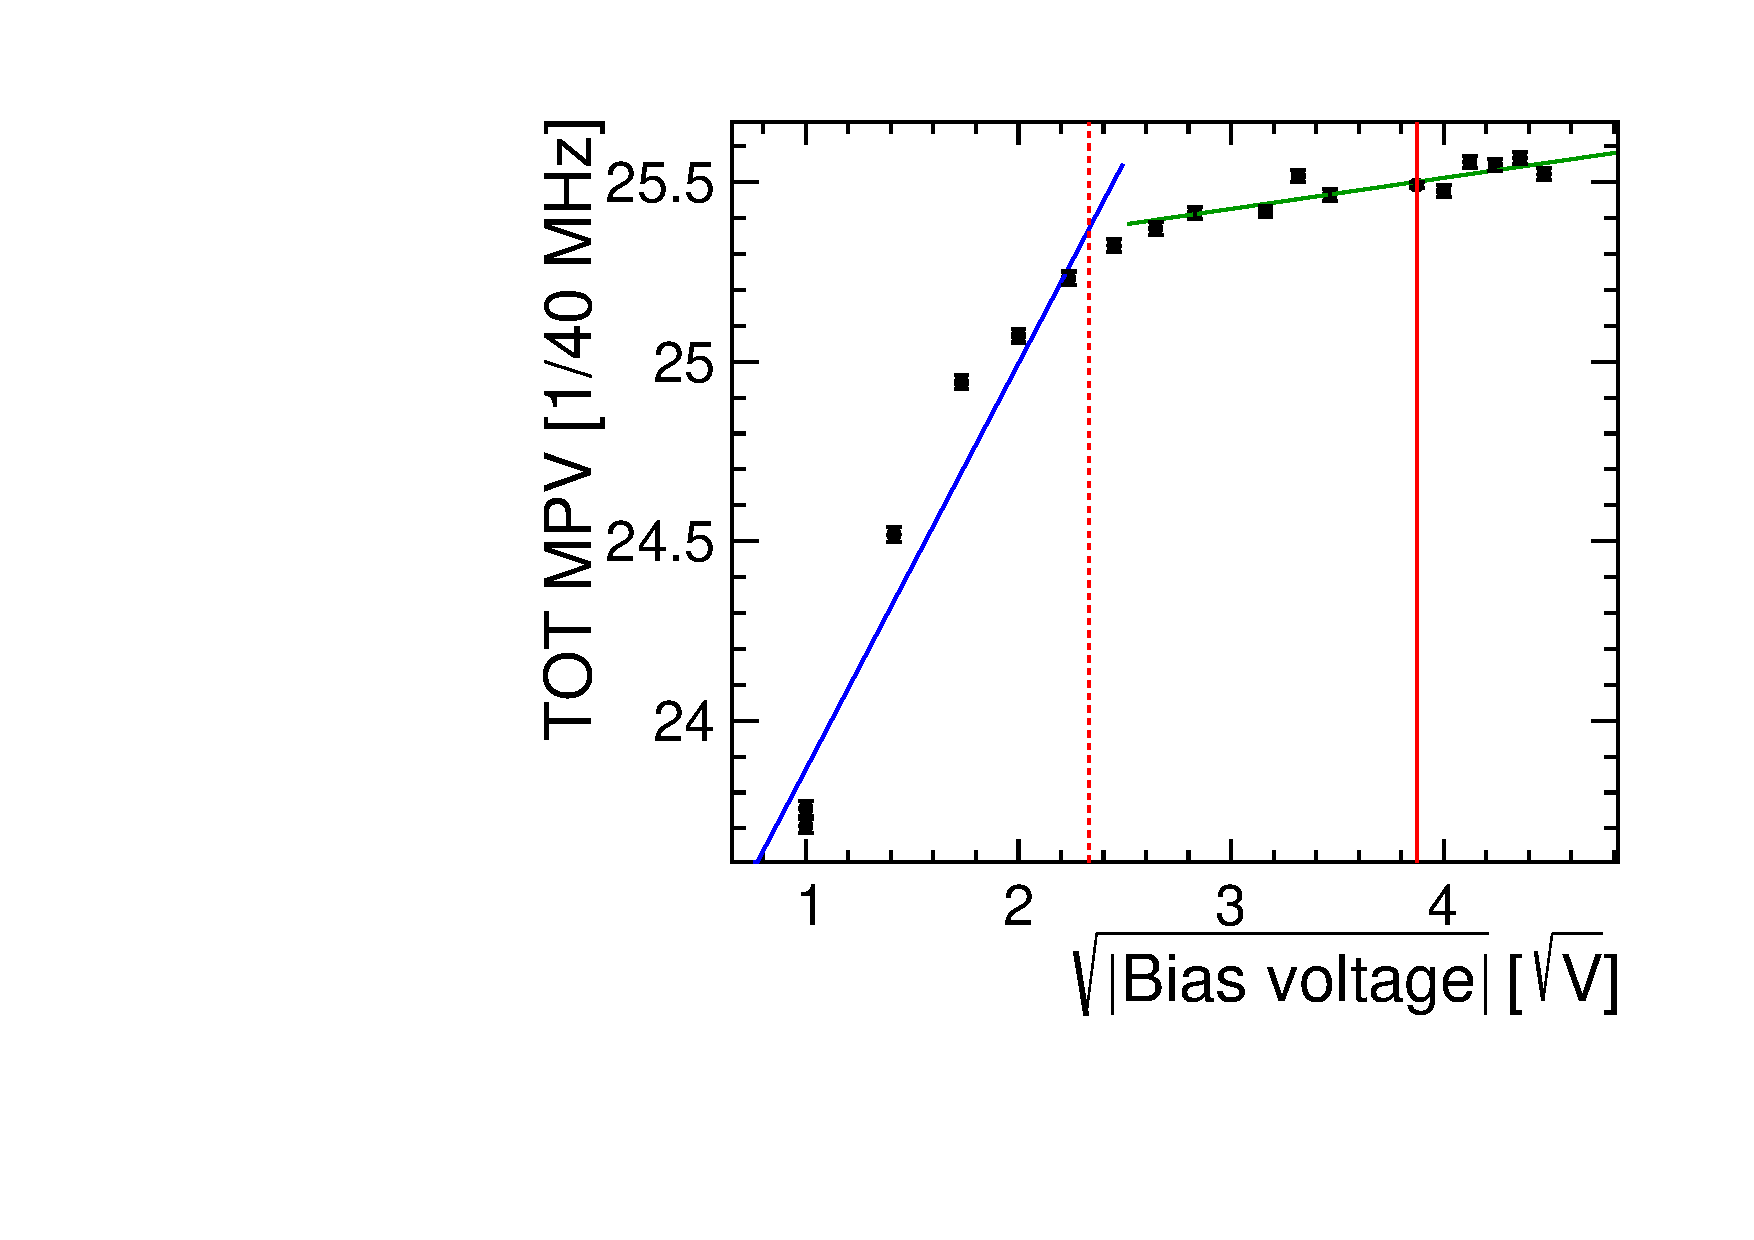
\includegraphics[width=\textwidth]{./figures/TestBeam/depletionVoltage_W0019_C07.pdf}
%%     \caption{}
%%   \end{subfigure}
%%   \caption{55-GNDGR (W19\_C7): bias and voltage scan.}
%%   \label{fig:Timepix3_THLscan_Vdep_C7}
%% \end{figure}

%% \begin{figure}[htbp] \centering
%%   \begin{subfigure}[b]{0.45\textwidth}
%%     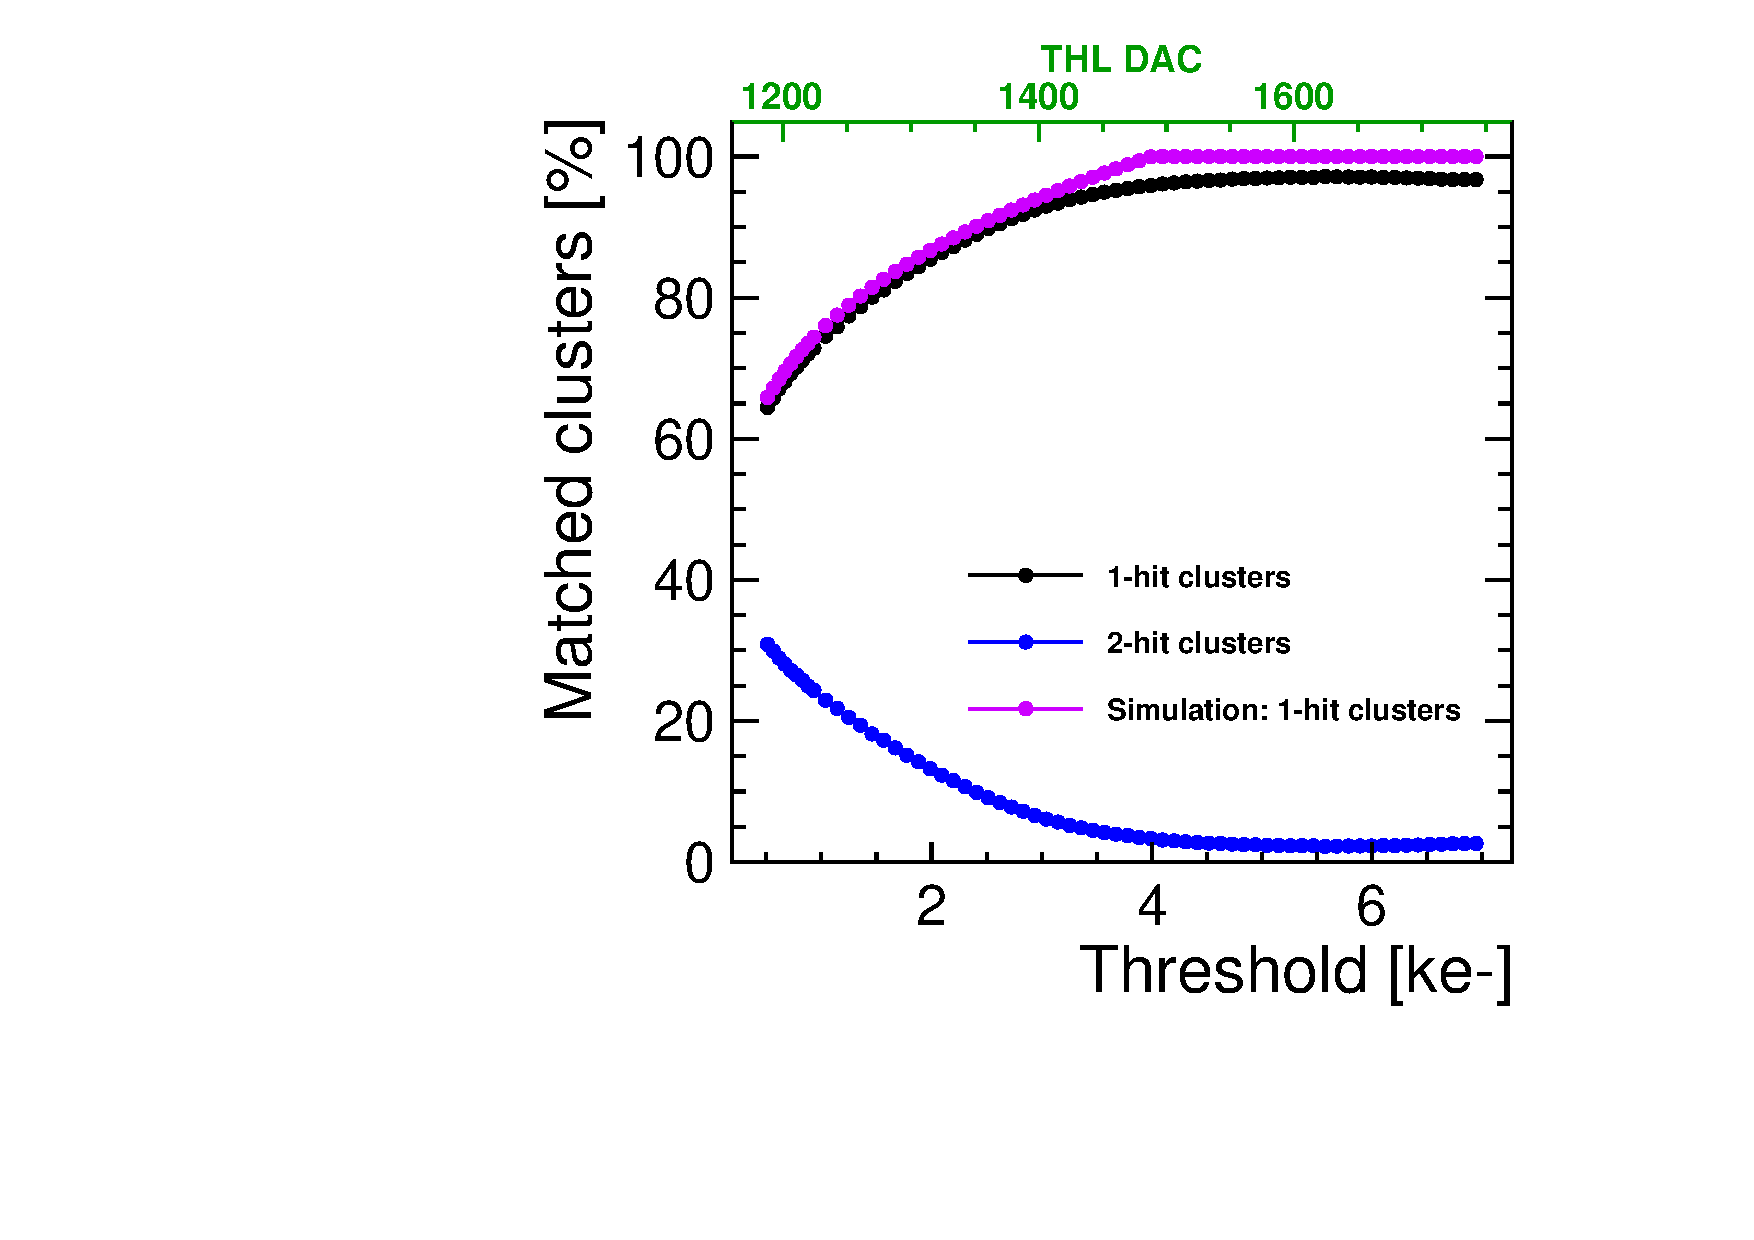
\includegraphics[width=\textwidth]{./figures/TestBeam/ThresholdScan_W0005_E02.pdf}
%%     \caption{}
%%   \end{subfigure} \hfill
%%   \begin{subfigure}[b]{0.45\textwidth}
%%     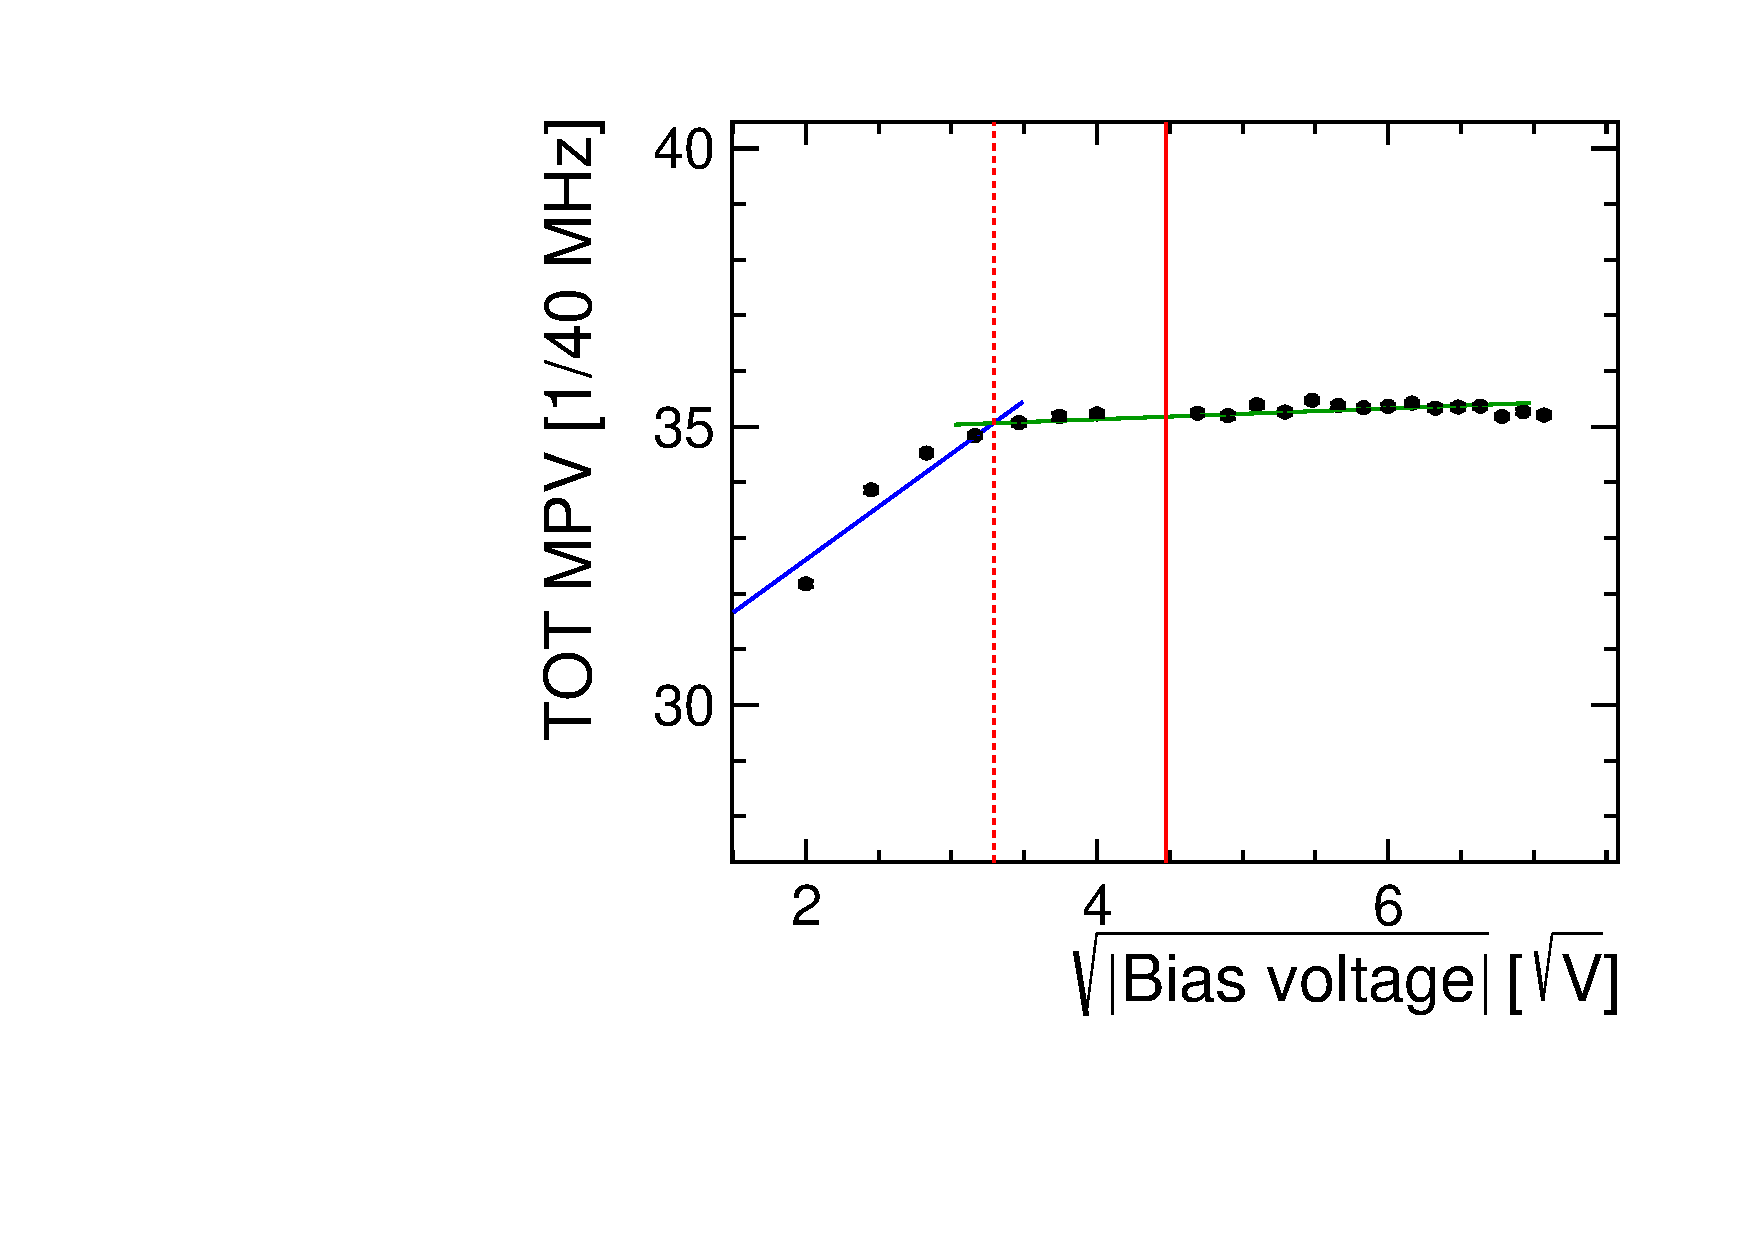
\includegraphics[width=\textwidth]{./figures/TestBeam/depletionVoltage_W0005_E02.pdf}
%%     \caption{}
%%   \end{subfigure}
%%   \caption{55-GNDGR-100 (W5\_E2): bias and voltage scan.}
%%   \label{fig:Timepix3_THLscan_Vdep_E2}
%% \end{figure}


%% \begin{figure}[htbp] \centering
%%   \begin{subfigure}[b]{0.45\textwidth}
%%     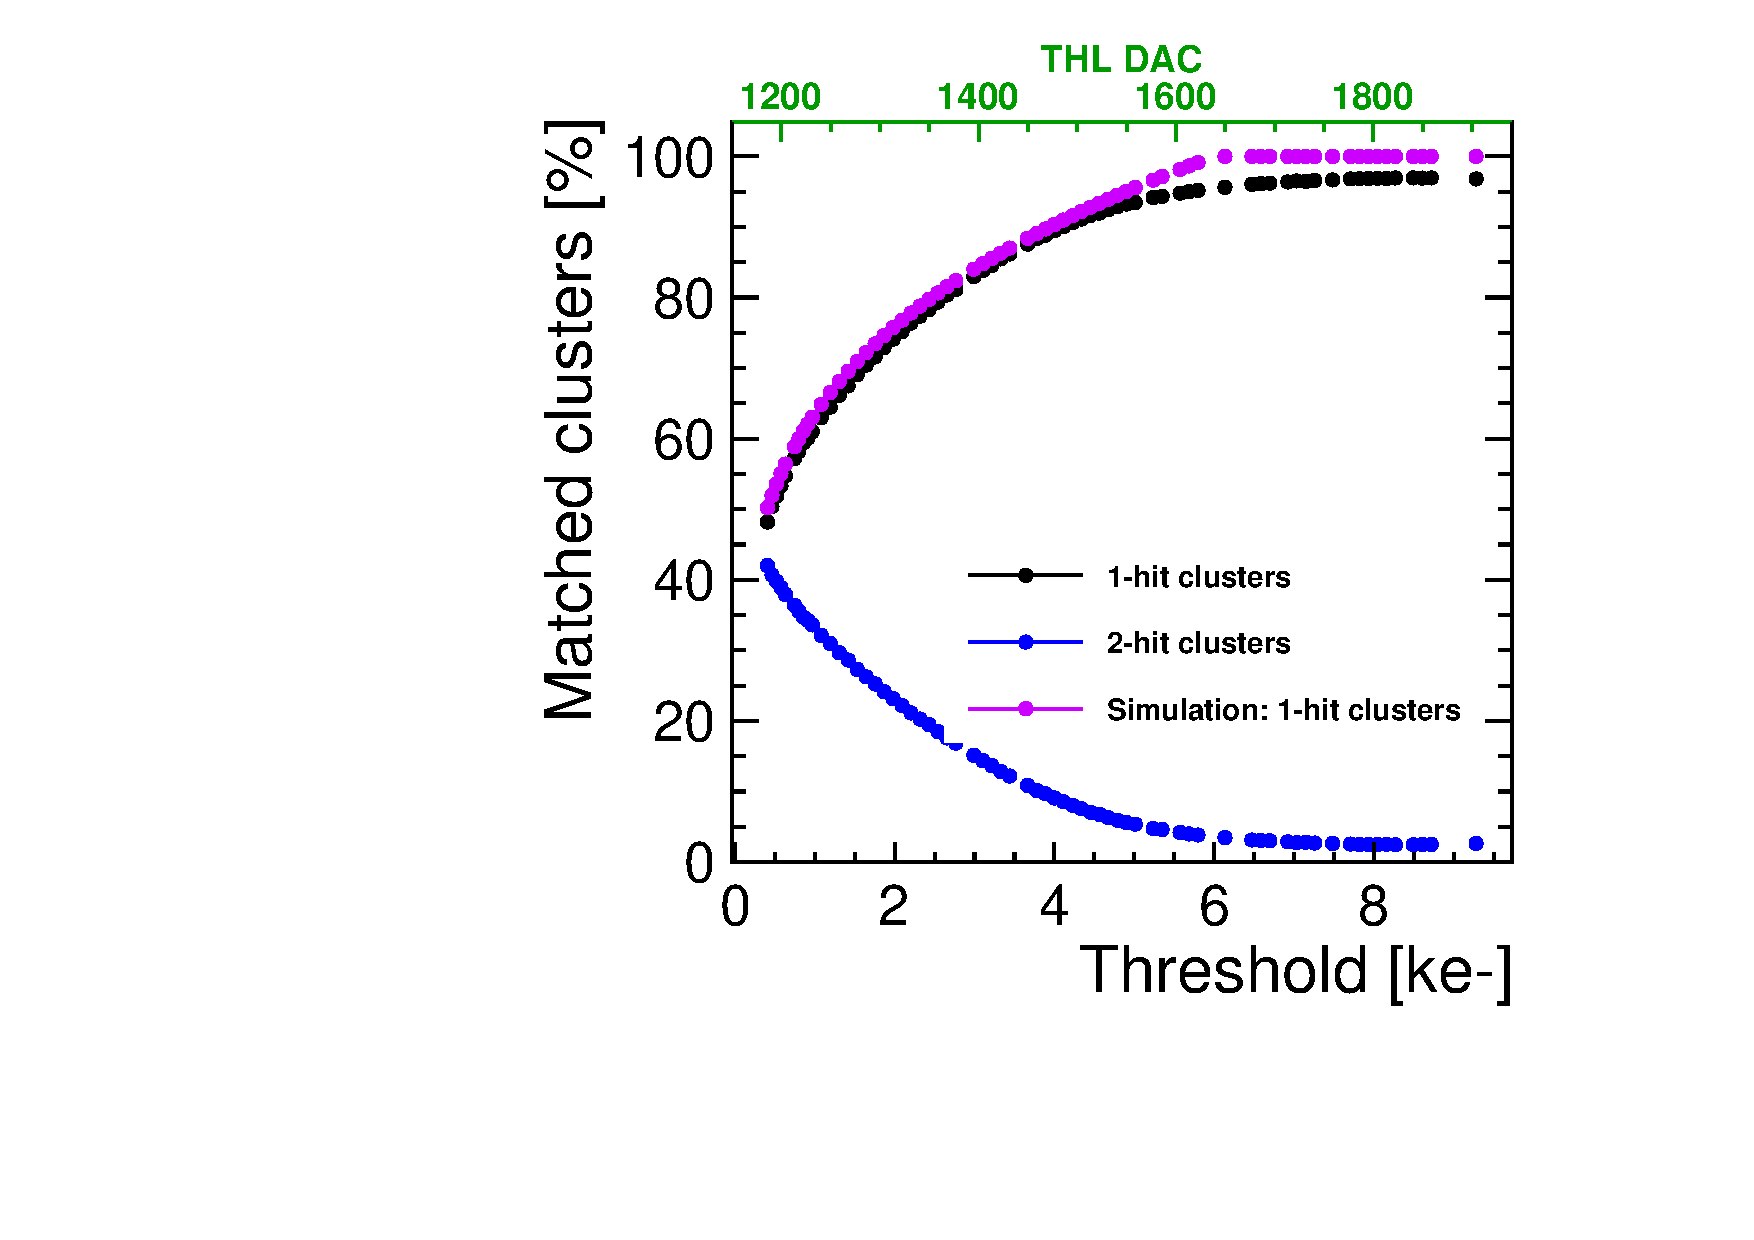
\includegraphics[width=\textwidth]{./figures/TestBeam/ThresholdScan_W0005_F01.pdf}
%%     \caption{}
%%   \end{subfigure} \hfill
%%   \begin{subfigure}[b]{0.45\textwidth}
%%     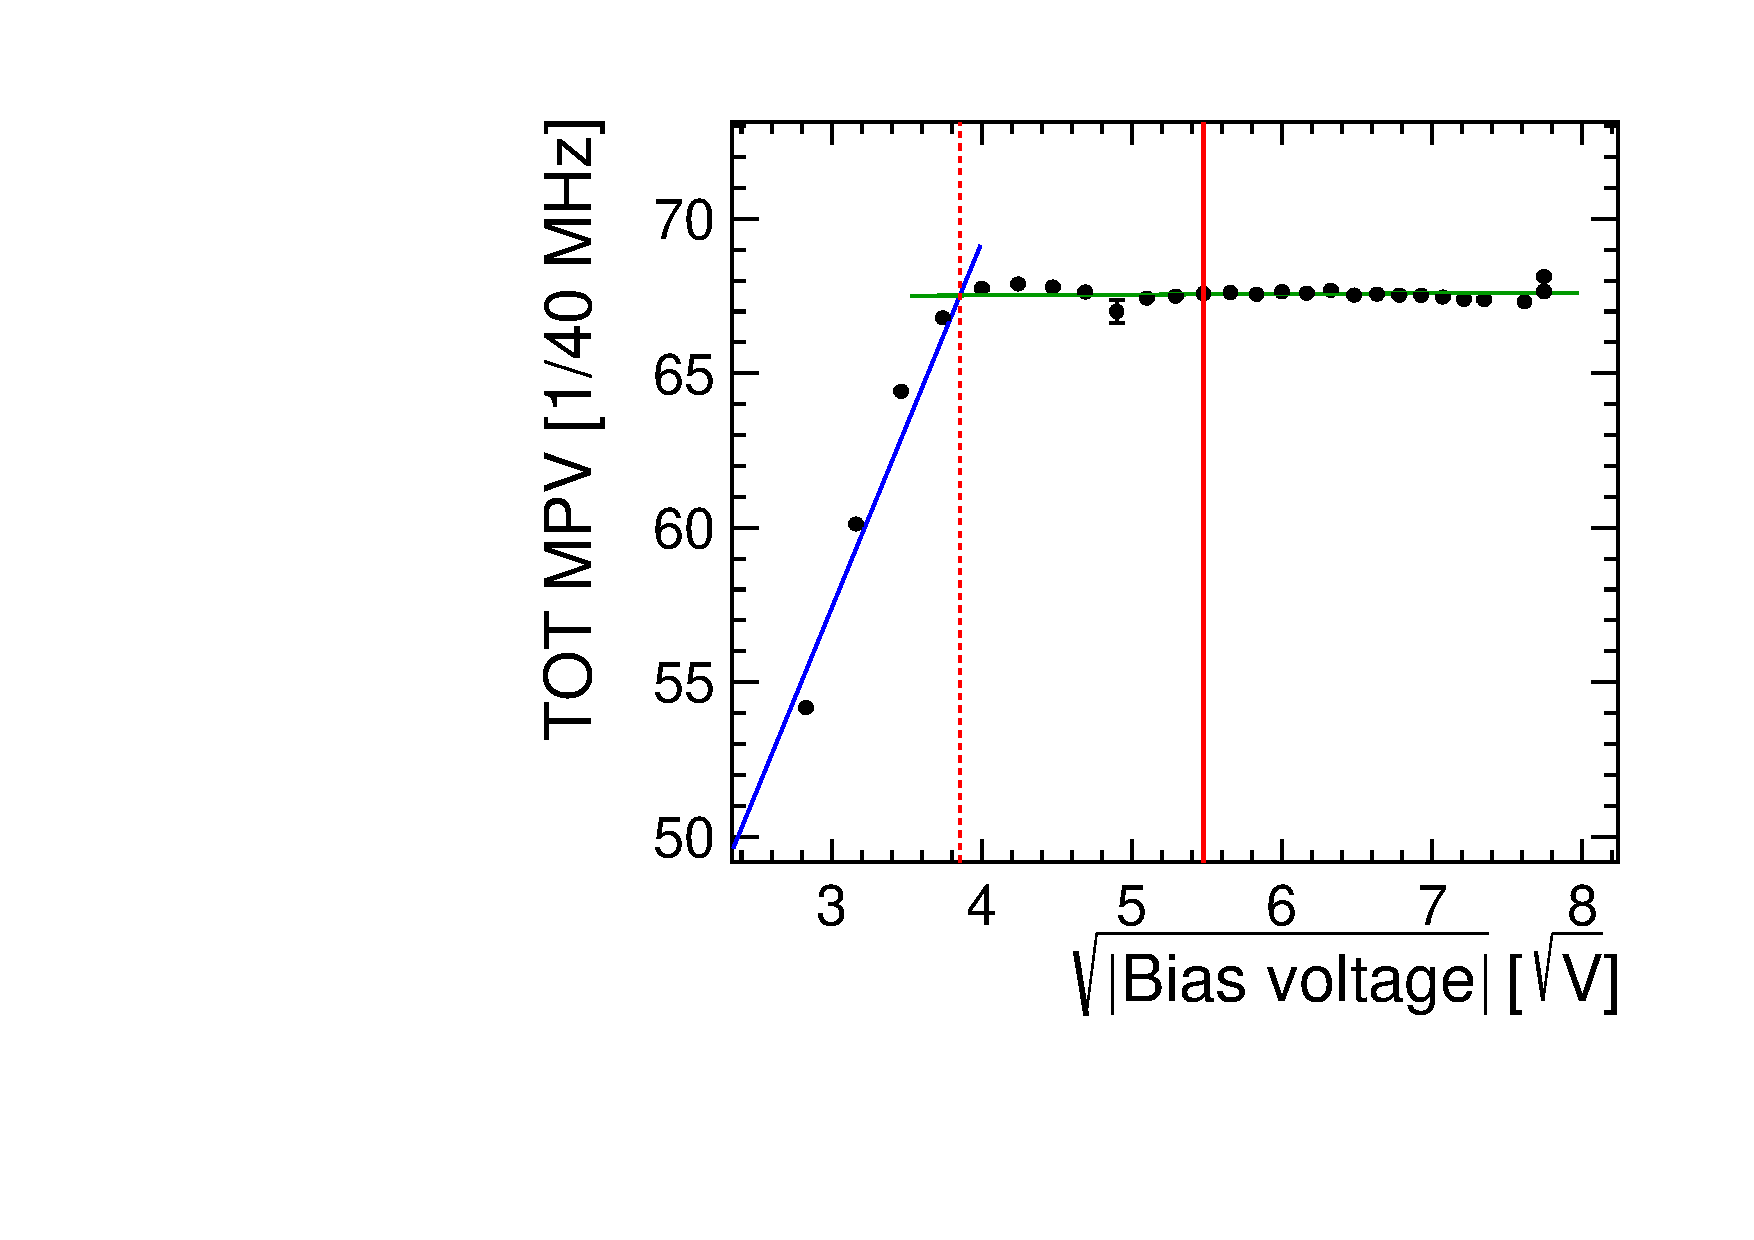
\includegraphics[width=\textwidth]{./figures/TestBeam/depletionVoltage_W0005_F01.pdf}
%%     \caption{}
%%   \end{subfigure}
%%   \caption{55-GNDGR-150 (W5\_F1): bias and voltage scan.}
%%   \label{fig:Timepix3_THLscan_Vdep_F1}
%% \end{figure}
